% \documentclass[a4paper,twoside]{article}
% \usepackage{fullpage}
% 
% 
% 
% 
% \usepackage[utf8]{inputenc}
% \usepackage[T1]{fontenc}
% \usepackage{RR}
% \usepackage{hyperref}
% 
% \usepackage{amssymb}
% \setcounter{tocdepth}{3}
% \usepackage{graphicx}
% 
% %%% Our Extra Packages %%%
% 
% %\usepackage{epic,eepic,amsmath,latexsym,amssymb,color,amsthm}
% \usepackage{ifthen}%,graphics,epsfig,fullpage} 
% 
% %%%
% 
% \usepackage{etoolbox}
% 
% 
% \usepackage{verbatim}
% \usepackage{graphicx}
% \usepackage{times}
% \usepackage{amsmath,amsfonts,amssymb,latexsym}
% %\usepackage{txfonts,pxfonts,wasysym}
% \usepackage{color}
% \usepackage{flushend}
% \usepackage{subfigure}
% \usepackage{multicol}
% \usepackage{hhline}
% \usepackage{cite}
% \usepackage[table]{xcolor}
% \usepackage{mathptmx}
% \usepackage{floatflt} 
% \usepackage{hyperref} 
% 
% 
% 
% 
% \usepackage{url}
% 
% 
% \newcommand{\ignore}[1]{}
% 
% %-----------------------for square--------------------------------------------
% \newlength {\squarewidth}
% \renewenvironment {square}
% {
% \setlength {\squarewidth} {\linewidth}
% \addtolength {\squarewidth} {-12pt}
% \renewcommand{\baselinestretch}{0.75} \footnotesize
% \begin {center}
% \begin {tabular} {|c|} \hline
% \begin {minipage} {\squarewidth}
% \medskip
% }{
% \end {minipage}
% \\ \hline
% \end{tabular}
% \end{center}
% }  
% %--------------------------------------------------------------------
% %--------------------------------------------------------------------
% %-------- macros for algorithm ---------------------------------------
% %\newtheorem{definition}{Definition}
% %\newtheorem{theorem}{Theorem}
% %\newtheorem{lemma}{Lemma}
% %\newtheorem{corollary}{Corollary}
% \newcommand{\toto}{xxx}
% %\newenvironment{proofT}{\noindent{\bf Proof }} {\hspace*{\fill}$\Box_{Theorem~\ref{\toto}}$\par\vspace{3mm}}
% %\newenvironment{proofL}{\noindent{\bf Proof }} {\hspace*{\fill}$\Box_{Lemma~\ref{\toto}}$\par\vspace{3mm}}
% %\newenvironment{proofC}{\noindent{\bf Proof }} {\hspace*{\fill}$\Box_{Corollary~\ref{\toto}}$\par\vspace{3mm}}
% 
% 
% \newcounter{linecounter}
% \newcommand{\linenumbering}{\ifthenelse{\value{linecounter}<10}{(0\arabic{linecounter})}{(\arabic{linecounter})}}
% \renewcommand{\line}[1]{\refstepcounter{linecounter}\label{#1}\linenumbering}
% \newcommand{\resetline}[1]{\setcounter{linecounter}{0}#1}
% \renewcommand{\thelinecounter}{\ifnum \value{linecounter} > 9\else 0\fi \arabic{linecounter}}
% 
% \newcommand{\tuple}[1]{\ensuremath{\left \langle #1 \right \rangle }}
% 
% %----------------------------------------------------------------------
% 
% 
% 
% 
% 
% 
% 
% %% d\'efinitions particulires  ce document %%%%%%%%%%%%%%%%%%%%%%%%%%%%%%%%%%
% % < mettre ici vos propres d\'efinitions \newcommand, \newenvironment, etc. > %
% %% fin des d\'efinitions particulires %%%%%%%%%%%%%%%%%%%%%%%%%%%%%%%%%%%%%%%%
% 
% 
% 
% \RRtitle{M\'emoire Transactionnelle: Imposer l'isolement forte entre transactions et op\'erations non-transactionnelle
% }
% 
% \RRetitle{ STM systems: Enforcing strong isolation between transactions and non-transactional code
% }
% 
% \RRauthor{         %% Le ou les auteurs %%%%%%%%%%%%%%%%%%%%%%%%%%%%%%%%%%%%
% \vspace{-1em}
% Tyler CRAIN\thanks[ur1]{IRISA, Universit\'e de Rennes 35042 Rennes Cedex, France}\and
% Eleni KANELLOU\thanksref{ur1}\and
% Michel RAYNAL\thanks{Institut Universitaire de France}\thanksref{ur1}
% \\
% {\it tyler.crain@irisa.fr, eleni.kanellou@irisa.fr, raynal@irisa.fr}
% }
% 
% 
% %% Champs pour les hauts de pages si diff\'erents du titre et des auteurs %%%%
% \authorhead{T. Crain, E. Kanellou \& M. Raynal}     %% auteurs : pages paires %%%%%%%%%%%%
% \titlehead{STM systems: Enforcing strong isolation between transactions and non-transactional code}      %% titre : pages impaires %%%%%%%%%%%%
% 
% \RRnote{         %% Note, contrat, collaboration, etc... %%%%%%%%%%%%%%%%%
% }
% 
% \RRdate{May 2012}         %% date de publication %%%%%%%%%%%%%%%%%%%%%%%%%%%%%%%%%%
%                    %% (si diff\'erente de la date systme %%%%%%%%%%%%%%%%%%%%
% 
% \RRNo{7970}           %% no du PI %%%%%%%%%%%%%%%%%%%%%%%%%%%%%%%%%%%%%%%%%%%%%
%                    %% (communique par le centre de doc )  %%%%%%%%%%%%%%%%%%
% 
% \RRresume{Ce rapport pr\'esente un algorithme de m\'emoire transactionnelle
% qui impose l'isolement forte entre transactions et op\'erations non-transactionnelle.
%         %% r\'esum\'e en franais %%%%%%%%%%%%%%%%%%%%%%%%%%%%%%%%%%%
% }                  %% fin du resume %%%%%%%%%%%%%%%%%%%%%%%%%%%%%%%%%%%%%%%%
% 
% \RRmotcle{m\'emoire transactionnelle, atomicité      %% Mots clef en franais %%%%%%%%%%%%%%%%%%%%%%%%%%%%%%%%
% }
% 
% \RRabstract{Transactional memory (TM) systems implement the concept of an atomic execution unit called  
% {\it transaction} in order to discharge programmers from explicit synchronization management. 
% But when shared data is atomically accessed by both transaction and non-transactional code, 
% a TM system must provide  {\it strong isolation} in order to overcome consistency problems.
% Strong isolation enforces ordering between non-transactional operations and transactions and 
% preserves the atomicity of a transaction even with respect to non-transactional code. 
% This paper presents a TM algorithm that implements strong isolation with the following features: 
% (a)  concurrency control of non-transactional operations is not based on locks and is particularly efficient, and 
% (b) any non-transactional read or write operation always terminates (there is no notion of commit\slash abort associated with them). 
%  %, TL2, Terminating Operation, Opacity, Non-transactional Operation, Consistency}   %% r\'esum\'e en anglais %%%%%%%%%%%%%%%%%%%%%%%%%%%%%%%%%%%%
% }                  %% fin de l'abstract %%%%%%%%%%%%%%%%%%%%%%%%%%%%%%%%%%%%
% 
% \RRkeyword{Transactional Memory, Strong Isolation, Atomicity       %% Mots clef en anglais %%%%%%%%%%%%%%%%%%%%%%%%%%%%%%%%%
% }
% \RRprojet{ASAP}
% \URRennes
% \RCRennes
% 
% 
% 
% 
% 
% \begin{document}
% 
% \makeRR

\section{Introduction}
\label{sec:SIintro}

Simplified transaction semantics may not be enough.
In the interest of ease-of-use, each chapter in this takes a 
different look on transaction semantics.
The first chapter suggested improving STM
protocols without changing the semantics of a transaction, the second
chapter suggested simplifying the semantics of a transaction,
and this chapter will suggest expanding the semantics.
It will look at how a programmer might use transactions
within his code in order to suggest the expansion of transactional
semantics in the interest of ease-of-use.

Following the discussion of the previous chapter we will promote our change
of semantics by contrasting transactions to concurrent objects.

A discussion on semantics the of concurrent protocols is meaningless without
first considering consistency conditions.
By satisfying a consistency condition a concurrent protocol allows the
user of that protocol to reason about how he can use it in his program
in a concurrent setting.
For example having a concurrent data structure that satisfies linearizability
means that the operations of a data structure will have a global order
based on the invocation and completion time of operations.
This allows, for example, a programmer who is coding some user based service
to use reasoning such as: if user $A$ who
is being serviced by thread $T_A$ changes his status to online (adding him
to the set of online users backed by a linearizable concurrent data structure)
then a following query for the names of online users
by user $B$ serviced by a different thread $T_B$ is guaranteed to contain
user $A$.
Without linearizability the programmer cannot necessarily use this reasoning, he might then
have to consider that the query by thread $T_B$ might or might not include $A$
leaving the programmer to have to come up with a solution for this.

Likewise in transactional memory, a correctness condition helps the
programmer reason about how he can use transactions in his programs.
For example opacity ensures that all transactions have a global order
and each transaction appears to have happened instantly at some point
in time between its invocation and committal.
This allows the programmer to create multi-process programs where the processes are
synchronized using programmer defined atomic operations.
The most common example of this is a banking application defined by transactions.
A programmer writing such a bank application may want to define an operation
that transfers a given amount of money $m$ from account $A$ to another account $B$.
In order to do this he creates a transaction that first reads the balance
on the source account ($A.balance$), and if the account has enough money the transfer
proceeds by first setting $A.balance$ to the value previously read minus $m$.
Next the balance of account $B$ is read, before setting its new balance
to the value read plus $m$ and the transaction is completed.
Given that the programmer uses an STM protocol that ensures transactions are executed
atomically, a user of this program will see only valid transfers
completed, otherwise conditions might arise where a balance is concurrently
modified by another process during a transaction, resulting in invalid balances
where someone could loose or gain too much money.

As the above examples illustrate, it is necessary for a concurrent protocol
to satisfy a clear and straightforward consistency condition in order
for a programmer to reason about how to use it.
% The previous chapter used the example of a universal construction for
% concurrent objects in order to movivate the design of a STM protocol
% with similar guarantees of progress.
% It also highlighted the diffrenece between an operation on a concurrent object
% and a transaction to show how the protocols differ in design.
% This chapter will use these difference to motivate an addition to the
% semantics of transactions.
Now we will suggest that due to the way transactions are used in a program
an STM protocol should satisfy more then just a correctness condition
such as opacity.
The reason for this is that opacity only considers the atomicity between transactions themselves,
and to motivate this suggestion we will go back to the comparison of
a transaction and an operation on a concurrent object.

For a concurrent object consider the common example of a tree
data structure implementing the set abstraction.
This abstraction might provide the following linearizable operations:
$insert(K)$ which adds $K$ to the set if it does not already exist, returning $true$
on success, $delete(K)$ which removes $K$, if it exists, from the set
returning $true$ on success, and $contains(K)$ returning $true$ if $K$
exists in the set, $false$ otherwise.
Here there are two important things to point out, first is that these operations
are contained to their data structure implementation, the status of shared
memory outside of the data structure has no affect on these operations.
Second is that these operations fully implement the desired abstraction
(in this case a set),
a user chooses to use this specific implementation because he needs
the $insert$, $delete$, and $contains$ operations.
If he wanted additional functionality such as in-order iteration, then
he would have to choose a different implementation providing the appropriate
abstraction.
This might lead the programmer to consider data structure as a separate entity
from that of the program where this entity is accessible through some fixed
interface, he need not be aware of the implementation below the interface.

Transactions on the other hand are integrated into the users program
rather then compromising some separate entity.
When a user places a transaction in his code it is because he requires
synchronization between the processes of his program, this synchronization
does not have to be based on some predefined abstraction or only access
some contained structure.
The concept of the transaction allows the programmer to be free to
perform any sort of operation, performing reads and write to any
location in the shared memory.
In this sense the transaction is a different type of mechanism
then a concurrent object as transactions are integrated and contained within
a user's program instead of being separate entities behind
a fixed interface.

So now we have concurrent objects whose operations follow some correctness condition
allowing them to be accessed as something interesting to the programmer as
a separate entity.
And transactions which appear as atomic blocks (thanks to the STM protocol
satisfying a correctness condition) built into a users program.
At a low level the difference between a transaction and an operation
on a shared object might imply separate protocol design choices.
For example the previous chapter highlighted some of the implementation
differences between a traditional universal construction and a
universal construction for transaction based programs.
But, let us step backwards for a moment and look at a higher level.
Before we consider implementation details we must consider how
how the programmer interacts with a transaction is considered at an abstraction level.
The previous discussion
has expressed the view that transactions exist as an integrated part of
a users program.
This happens when the programmer places a group of reads and writes
inside a block of code bounded by the keywords $transaction\_begin$ and
$transaction\_end$.
This atomic operation exists directly as a piece of his code preceded
and followed by code also written by himself.
% Inside this block of code reads and writes to shared memory are then
% treated by the STM protocol as calls to the operations
% $transaction\_read$ and $transaction\_write$.
% The STM protocol then
% takes care of the difficult synchronization in order to ensure these transactions
% appear as if they happen atomically.
At this point we have an important choice to make dealing with the
semantics and correctness of a transaction when considering shared memory.
Should the transactions appear to be atomic only with other transactions, or should
concurrent non-transactional shared memory accesses also be considered?
More precisely, should the shared memory that is accessed from within a transaction
be only safely accessible from within transactions, or should it be
safe to access memory inside and outside of transactions at any time,
or should it be something in-between?

Interestingly, this possibility of the {\it existence of two different paradigms} reveals
%between strong and weak isolation reveals 
two different interpretations of transactional memory: On one hand considering TM as an implementation
of shared memory, and, on the other hand, considering TM as an additional way of achieving synchronization, 
to be used alongside with locks, fences, and other traditional methods.
When putting ease-of-use as the primary requirement of transactional memory
as well considering the discussion on transactions vs operations on concurrent objects
the choice of paradigm seems clear.
If within a program there are two sets of shared memory, one set for accessing inside
transactions, and another set for accessing outside of transactions, then we loose a
bit of the integration concept for a bit more of the separated object concept.
One way to think of it is that the transactions represent a programmer defined
interface to one large discrete shared object.
Transactions are still defined and placed by the programmers, but they are limited
in what memory they can access.
On the other hand if the programmer can access shared memory both inside and outside
of transactions while the system is still ensuring the atomicity of the transactions then
we have a more straightforward integrated system.

\subsection{Transaction vs Non-transactional Code.}
\label{sec:TvNT}
Let us now define precisely what we mean by transactional vs, non-transactional
accesses.

In a  concurrent environment,  shared memory  may  be
accessed by both transactions as well as  
non-transactional operations. %This  is mostly brought about by  the need to
%continue using legacy code that existed before  
%transactional memory was  implemented.
In this work we consider that shared memory can be accessed through
reads and writes either inside or outside of transactions.
A read (respectively write) performed inside a transaction is consider
a transactional read (transactional write) while a read (resp. write)
performed outside a transaction is considered a non-transactional read
(non-transactional write).

The next section will discuss previous solutions on how to deal
with concurrent accesses to shared memory inside and outside of transactions
and where we think they fall short on the ease-of-use objective.

\subsection{Dealing with transactional and non-transactional memory accesses}
\label{sec:SIsolutions}
% Like dealing with aborted transactions there are several ways to deal
% with concurrent memory accesses inside and outside of transactions each
% with different implication on how the programmer uses STM.

\paragraph{Weak isolation}
STM protocols implementing \emph{weak isolation} make no guarantee
about concurrent transactional and non-transactional memory accesses.
Transactions are considered to  
happen atomically only with respect to other transactions.  Given this, it is possible
for non-transactional operations to see intermediate results  
of transactions that are still  live. Conversely, a transaction may see the
results of non-transactional operations that happened during  
the  transaction{}'s   execution.
% If  this  behavior   is  not  considered
% acceptable for an application, then the responsibility to prevent it is  
% delegated   to  the   programmer  of   concurrent  applications   for  this
% system.
Nevertheless, these concurrency issues can be anticipated and used
appropriately by the 
programmer,  still resulting  in correctly  functioning  applications.
Ways of how a programmer might consider to use weak isolation in his code
is presented in \cite{blundell06}.
This requires the programmer 
to  be conscious  of  eventual race  conditions  between transactional  and
non-transactional code that can change depending on the STM system used.
Not only can this make transactional code extremely difficult to write
and understand, but a simple change in the STM protocol could render the
program useless.
Obviously this is not a good solution to concurrent transactional and non-transactional
access when considering ease-of-use.

More commonly, an STM protocol that implements weak isolation expects users to avoid
any concurrent interaction between the shared memory outside and inside of
transactions.
This is because the type of consistency guaranteed is usually undefined
and depends on the implementation of the STM protocol used.
A programmer already has to consider different types of memory such as thread local
process local and shared memory so having him decide what memory should be transactional
and what should not be just adds an additional burden to the programmer.
Along with this, having a separate section of memory for transactions is also not consistent with
the concept of transactions being integrated within a program.

Therefore, in order  to keep consistent with  the spirit of TM  principles a
system should prevent unexpected   results  from   occurring  
in presence of  race conditions. 
Furthermore, concurrency   control should  ideally be implicit  
and never be delegated to  the programmer~\cite{CIR12,MS12}.
It is for these reasons that when considering transactional and non-transactional accesses
we want something stronger then weak isolation in order to keep things
as simple as possible for the programmer.

It is important to note that most current high performance STM protocols implement weak isolation
as providing stronger guarantees tend to have an impact on performance.

% Under weak isolation, transactional and non-transactional operations can be
% concurrent, but the programmer has to be aware of how to handle these.


\paragraph{Specialized transactions}
In some cases a programmer using an STM that satisfies
weak isolation can deal with concurrency issues between transactional
and non-transactional accesses himself.
Usually a programmer will purposely subject himself to these
difficulties in the interest of performance.
Examining more formally these performance over ease-of-use concepts, several
STM protocols have been proposed allowing the existence of transactions
that might not appear as being atomic.
These protocols often focus on ways to give the programmer the power to weaken the semantics
of certain transactions or even specific reads within transactions.
DSTM \cite{HLMS03} introduced the concept of \emph{early-release}, giving a programmer
the ability to remove locations from the read set of a transaction,
in the hope of improving performance by lessening the likely-hood of a
transactional abort.
\emph{Elastic} transactions \cite{FGG09} allow a programmer to mark transactions that
satisfy a weaker consistency condition then opacity allowing for efficient
implementations of search data structures.
While this chapter focuses on the interaction between shared memory accesses
inside and outside of transactions, we felt it was interesting to mention
these solutions as in a way they allow a sort of non-transactional read
to be preformed from within a transaction.

\paragraph{Privatization}
Privatization is an interesting solution problem to the splitting of memory
between transactions and non-transactional accesses.
As the name implies, privatization gives the programmer the ability
to privatize sections memory to a specific process giving it exclusive access to
memory that was previously shared.
The programmer does this through the use of what is called a privatizing transaction
within which he makes some memory unaccessible from other processes' transactions.
Once a process has privatized some memory then is safe
to access it outside of transaction within the privatizing thread.
After privatization, memory can then be publicized to be accessed
from within transactions again
by using a publication transaction.

A typical  example of privatization would  be the manipulation  of a shared
linked list. The  removal of a node $n$ by a  transaction $T_i$, for private
use, through  non-transactional  code,  by  the process $p$ that  invoked $T_i$,  
constitutes  privatization. Then, $T_i$  is called privatizing transaction. 
Obviously after the transaction commits future transactions will no longer
be observe $n$ in the list, but unless the STM protocol is privatization safe
$p$ cannot safely access $n$ non-transactionally.
Normally this is due to the fact that there could be live transactions
that started before $T_i$ committed who have concurrently accessed $n$.
% While the privatization is not visible to all processes, inconsistencies may arise, given 
% that for $T_i${}'s process the node is private but for other processes, the node is 
% still seen as shared. 
These problems are closely examined in \cite{spear07}.
Here they show that providing privatization safety is not as
simple as just implementing an STM protocol that provides opacity as incorrect results due to
privatization can occur regardless of the update policy
(redo log or undo log)  that a  transactional memory algorithm implements. 
As  an example, consider
the cases that result when given two processes $p_1$ and   
$p_2$ that privatize shared variable $x$:
\begin{itemize}
\vspace{-0.1cm}
\item  
The TM implementation  uses a  redo log.  Process $p_1$ privatizes  $x$ with
privatizing transaction $t_1$ but stalls before committing $t_1$.  
$p_2$ executes during this stall and will not see the effects of $t_1$. 
$p_2$ proceeds to privatize $x$ itself and to access it through 
non-transactional operations. The variable $x$  will still be accessed through 
transaction $t_1$ when process $p_1$ resumes and the results of $p_2$'s 
privatization will not be visible to it. 
\vspace{-0.2cm}
\item The TM implementation uses an undo log. As above, $p_2$ privatizes 
$x$ but $p_1$ stalls before performing validation before attempting 
to commit. In the meanwhile, $p_2$ executes, privatizes $x$ and commits. 
Given that updates are done in-place, $p_2$ will observe the updates 
performed by $t_1$. However, when $t_1$ resumes and attempts to commit, 
its validation will fail and it will abort. $p_2$ will be left privately 
accessing data that are no longer valid.
\end{itemize}


\anote{Need to put in citations for these, update this paragraph}
Several solutions have been proposed for the privatization problem 
such as using visible reads, conventional means of 
synchronization such as fences, sandboxing, partitioning by consensus 
\cite{scott07}, the use of lock-free reference   counters   \cite{afek10}  or   
by  using private transactions \cite{dice10}, to name a few. 
Several protocols implementing privatization have been proposed,
ranging from solutions where a programmer uses a special keyword to mark
which transactions are privatizing, to others that ensure safety by having
a privatizing transaction block until all other concurrent transactions
have finished, to more complex non-blocking solutions.


A main advantage of privatization is in the case of performance, as when
a thread privatizes some memory, it can then access it without overhead.
While privatization is an interesting solution, we feel that is does not
fit in our model of ease-of-use for two main reasons.
Firstly the separation between the memory safe to access by transactions
and that safe to access outside of transactions is still separated, privatization/
publication just gives the user the ability to dynamically move sections of memory
from one part to another.
Secondly it adds an extra layer of complication to the transactional memory
abstraction, if the programmer wants to takes advantage of privatization he
has to decide when and what to privatize and publicize.



%In  a  system  that  does  not  provide  strong  isolation,  unsynchronized
%concurrent access can occur between two processes on a memory  
%area that both  view as shared. However, it can also  occur on memory areas
%that one of the threads views as shared while the other  
%considers them to  be its private memory area. 
%Another area where synchronization between transactional and 
%non-transactional code is needed, is the referred to  as the

% A discussion of the co-existence of transactional and non-transactional code 
% would not be complete without mentioning the
% {\it privatization problem}.
% An area of shared memory is privatized,  
% when a process  that modified it makes it  inaccessible to other concurrent
% processes\footnote{Conversely, a memory area is made public  
% when it goes from being exclusively accessible by one process to being 
% accessible by several processes \cite{spear08} . 
% This is referred  to as the {\it publication problem} and the consistency 
% issues that arise are analogous.} with the purpose being
% that the process can then access
% the memory without using synchronization operations \cite{spear07}.  







\paragraph{Solution from scott/spear}
\anote{Need to write and cite}

\paragraph{Strong isolation}

\emph{Strong isolation}, in order to spare the programmer from the responsibilities
raised by weak isolation or privatization, ensures that  
both the  transactions  and  the non-transactional
read and write operations are be implemented in a way  
that  takes their co-existence  into account.
% Such an  implementation that
% provides synchronization  between transactional and  non-transactional code
% is said to provide strong isolation.
Strong isolation ensures that the non-transactional accesses to shared memory
do not violate the atomicity of the transactions.
As a result,
the aforementioned scenarios described in the paragraphs about weak isolation
and privatization  where non-transactional operations  violate
transaction isolation, are not be allowed to happen.  
In fact strong isolation
inherently also solves the privatization problem as it
imposes synchronization between transactional and non-transactional code.

In order to better understand strong isolation guarantees, consider
the following simple intuitive extension that can be applied to an STM protocol
in order to ensure strong isolation.
In order to provide this extension, any non-transactional operation that 
accesses shared data is simply treated as a ``mini-transaction'', i.e., a transaction  that contains a
single read/write operation. In that case,  transactions  will have to  be  
consistent (see Sect.~\ref{sec:badthings})  not only with 
respect to each other, but 
also with respect to the  non-transactional operations.
Obviously in this solution there is no separate section of memory for transactions
and their atomicity is preserved resulting in a simpler framework for
the programmer then privatization or weak isolation.
While this solution is simple, it is not necessarily optimal performance wise.
As such, several more efficient approaches to implementing strong isolation have been proposed,
in \cite{shpeis07} a blocking implementation to strong isolation
is described by placing barriers in transactions to ensure safety.
In the interest of improving performance, this paper also proposes ways of performing dynamic
and static analysis in order to remove certain barriers
while still ensuring safety.
Further dynamic optimizations proposed in \cite{SMSA08}, but
even considering the most efficient implementations, strong isolation has been suggested to be too costly \cite{DS09}.
Other work has considered strong isolation in hardware transactional memory \cite{MTCM07}.
% TM has to guarantee that transactions will be isolated from each other, but
% when it  comes to transactions and non-transactional  operations, there are
% two  paths a  TM system  can follow:  it may  either act  oblivious  to the
% concurrency between transactions and non-transactional 
% operations, or  it may  take this concurrency  into account and  attempt to
% provide     isolation    guarantees    even   between    transactional   and
% non-transactional operations. The first  case is  referred to as \emph{weak
% isolation} while the second case is referred to as \emph{strong  
% isolation}.

When implementing strong isolation in order to ensure the safety of non transactional reads and writes
(weather they are implemented as mini-transactions or by using memory barriers)
they become more then just a single load or store operation when actually being executed on the processor.
In order not to increase the complexity of using transactional memory we want the programmer to be
able to perform non-transactional operations in his code just as he would a normal read and write.
This means at some point after the programmer has written the code and before it is executed
the additional operations must be added.
For example in \cite{shpeis07,SMSA08} memory barriers are added before non-transactional reads and writes
by the compiler.
This can also be done dynamically at runtime.

\paragraph{Precisely Defining Strong Isolation.}

The  distinction  of isolation guarantees  was  originally  made  in
\cite{blundell06},  where   reference  was  made   to  {}``weak
atomicity'' versus {}``strong atomicity''.
Interestingly this paper also presents examples of code that a programmer
might write to run along with an STM protocol that provides some type of weak
isolation which would not run using an STM protocol that provides strong isolation,
further suggesting that a standard should be proposed so that the programmer
is not stuck having to understand the intricacies provided by different STM
protocols.

Further complicating things, there  are different  definitions in  literature for  strong 
isolation \cite{blundell06,ma07,harris06}.
In this paper we consider strong isolation to be the following:
%\begin{enumerate}
%\vspace{-0.1cm}
%\item   Non-transactional   operations   are   considered   as ``mini''
%transactions which never abort and  contain only a single  read or 
%write operation. 
%\vspace{-0.2cm}
%\item The consistency condition for transactions is opacity.
%\end{enumerate}
%As non-transactional read an write operations never abort, 
%this is called {\it terminating strong isolation} in the following.
(a) non-transactional   operations   are   considered  as ``mini''
transactions which contain only a single  read or 
write operation, and (b) the consistency condition for transactions is opacity
(or virtual world consistency).
We choose this definition as it is simple and keeps with the spirit of atomic transactions
without having to separate the memory.
 
Using this definition, the properties referred to as
{\it containment}  and {\it non-interference} are satisfied.
These properties were defined in \cite{blundell06} in order to describe
the synchronization issues between concurrent transactional and non-transactional operations.
Containment is   illustrated in  the  left  part of  Fig.
\ref{fig:int-nonc}.  There,
under strong  isolation, we have  to assume that transaction  $T_1$ happens
atomically,  
i.e.,``all  or  nothing'',   also  with  respect  to  non-transactional
operations. Then, while $T_1$ is  alive, no non-transactional read, such as
$R_x$, should be  
able to obtain  the value written to $x$  by $T_1$. Non-interference
is  illustrated  in  the right part of Fig.  \ref{fig:int-nonc}.  
Under  strong  isolation, non-transactional  
code   should  not  interfere   with  operations   that  happen   inside  a
transaction. Therefore, transaction $T_1$ should not be able to observe the
effects of  operations $W_x$ and $W_y$, given that they happen concurrently with it, 
while no opacity-preserving serialization of $T_1$, $W_x$ and $W_y$ can be found. 
Non-interference violations can be caused, for example,  by non-transactional 
operations that are such as to cause the ABA problem for a transaction that has 
read a shared variable $x$.
% Non-interference of  a transaction  $T_1$ can also  
% be compromised  by the interaction between non-transactional  operations  and  
% another  transaction   $T_2$. 

\begin{figure*}[ht]
\centerline{
     \mbox{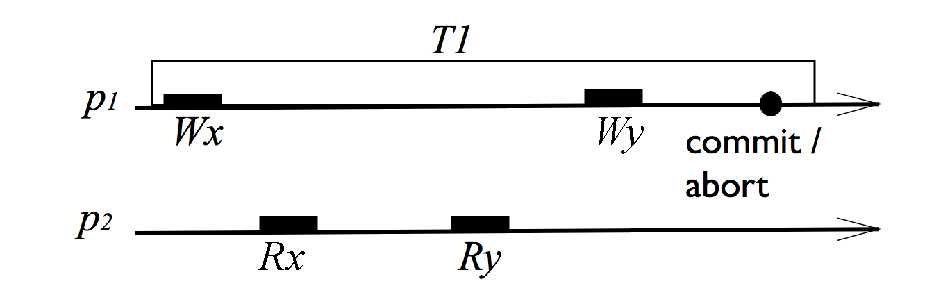
\includegraphics[width=0.4\textwidth]{SI/imgs/non_containment}}     
		%\mbox{\fig{file=imgs/non_containment, width=0.5\textwidth, clip=}}
    \mbox{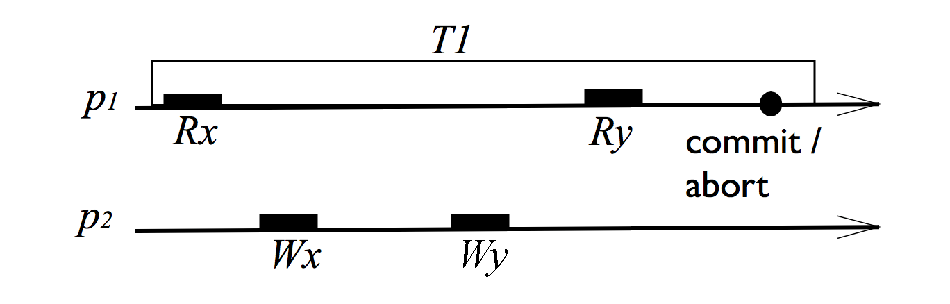
\includegraphics[width=0.4\textwidth]{SI/imgs/interference}}
		%\mbox{\fig{file=imgs/interference, width=0.5\textwidth, clip=}}
}
\caption{Left:  {\it Containment}  (operation $R_x$  should not  return the
    value written to $x$ inside the transaction). 
Right:  {\it  Non-Interference} (wile  it is still  executing, transaction
$T_1$ should not have access to the values that were written to $x$ and $y$
by process $p_2$).} 
\label{fig:int-nonc}
\end{figure*}
%An additional feature of strong isolation, implemented in this paper, 
%is that non-transactional read and write operations never abort. 
%For this reason, it is termed {\it terminating strong isolation}.


%Consider the
%case where a transaction $T$  
%pertaining  to process  $p_1$  reads variable  $x$  through read  operation
%$R_x$, and finds that it contains value  
%$v_1$.  Before $T$  commits, and  after  $R_x$ has  completed, assume  that
%another process $p_2$ modifies $x$  
%by  writing value  $v_2$ to  it through  non-transactional  write operation
%$W_{1x}$. Then, assume that either the  
%same process  $p_2$ or a different process  $p_3$ write non-transactionally
%value $v_1$ to $x$ through operation  
%$W_{2x}$. In  this case, process  $p1$ should have  a means to  detect this
%occurrence and transaction $T$ should  
%not commit, given that otherwise, strong isolation would be violated. 


%Non-interference for  a transaction  $T_1$ can also  be compromised  by 
%interaction between non-transactional  
%operations  and  another  transaction   $T_2$,  as  illustrated  in  Fig.
%\ref{fig:timent}. There, non-transactional operation  
%$R_{2x}$  reads  what transaction  $T_2$  has  written  to shared  variable
%$x$. Due to maintaining consistency, it is not  
%possible  to find  a  correct serialization  order where  non-transactional
%operation $W_y$ does not happen during the  
%duration  of transaction $T_1$,  violating non-interference.  Therefore, in
%order to preserve opacity, this situation would  
%have to  be detected when  transaction $T_1$ attempts to  execute operation
%$R_y$ and $T_1$ would have to be aborted. 
 

%\begin{figure*}[ht]
%\centerline{
%    \mbox{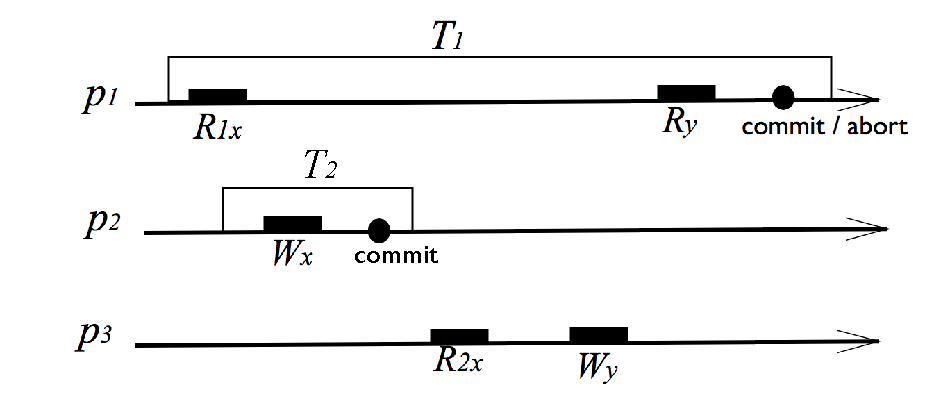
\includegraphics[width=0.5\textwidth]{imgs/time_NT.eps}}
%}
%\caption{Transaction  $T_2$  and  non-transactional operations  of  process
%$p_3$ interfere with transaction $T_1$.} 
%\label{fig:timent}
%\end{figure*}





%========================================================================
\subsection{Terminating Strong  Isolation}
\label{sec:protocol}


Strong isolation allows transactions to not be restricted to use a fixed
subset of memory while still ensuring their atomicity with respect to
other transactions as well as non-transactional operations.
This allows the programmer to preform reads ands write to the same memory he accesses
in his transactions without having to worry about observing or creating inconsistencies.
As indicated in the paragraph on strong isolation, one possible implementation
is to simply convert all non-transactional reads and writes into mini-transactions.
Let us also consider the solution to  the problem of  ensuring strong isolation 
by using  locks or barriers: Each shared
variable would then  
be associated with a lock and both transactions as well as non-transactional 
operations would have to access the lock before accessing the variable.
Locks are already used  in TM algorithms - such as TL2  itself - where it is
however     assumed   that  shared   memory   is   only  accessed   through
transactions. The use  of locks  in a TM algorithm  entails blocking and may
even lead a process to starvation.
Previous research on STM protocols has taken the approach that
these characteristics might acceptable.
The reason for this is that the
programmer  accepts the fact that a  transaction has a duration and that it
may  even  fail: Given that every live transaction has the possibility
to abort means that the  
failure to complete can be considered a part of the transaction concept.  

Now if we have non-transactional operations that rely on the same mechanisms
(either implemented using locks or by mini-transactions) then they are susceptible
to the same possibility of non-completion.
However one must consider that a transaction does not have the same semantics
as a simple read or write operation.
While the concept of the memory  transaction includes the possibility of failure,
the concept of a simple read/write operation does not.
When it  comes to single read or  write accesses  to  a shared
variable, a  non-transactional operation is normally understood  as an
event  that  happens   atomically  and   completes.
While executing, a  read  or write  operation   is  not 
expected  to  be de-scheduled, blocked or aborted.  
Unfortunately   strong
isolation  implemented with  locks  entails the blocking  
of non-transactional read and write operations and would not provide termination.
In the previous chapter we argued that, when considering ease-of-use, 
every transaction should be committed and the
possible non-termination of transactions is unacceptable.
Even worse would be if a programmer had to consider that simple
read and write operations to shared memory are not guaranteed to terminate.
Such an approach to strong isolation would then be rather counter-intuitive for the 
programmer (as well as possibly detrimental for program efficiency).

For this reason we believe that an STM protocol implementing strong
isolation should also consider the progress of non-transactional operations.
In order to deal with this we suggest that a STM protocol should implement
\emph{terminating strong isolation}, which we simply define as strong isolation
with the additional guarantee that the non-transactional read and write
operations of a process are guaranteed to terminate no matter the actions of
concurrent processes in the system.
The rest of this chapter will focus on the design of an STM protocol
that ensures terminating strong isolation.

% The non-transactional read and write operations in this algorithm
% focus on efficiency and do not
% rely on locks, instead only executing non-blocking operations with no loops
% ensuring their termination.







% This means that a
% programmer expects  that a transaction  
% might fail,  either by blocking or by  aborting.
% 
% read or write operations, which  the programmer expects to
% be  atomic. 





%Strong isolation always imposes synchronization between 
%transactional and non-transactional code that access memory areas that 
%are potentially shared, which means that a system that guarantees strong 
%isolation is inherently privatization safe.







% \paragraph{Content of the Paper.}
% This paper presents  a TM  algorithm which takes the
% previous issues into account. It is built on top of 
% TM algorithm TL2 \cite{dice06},  a  word-based  TM algorithm  that  uses locks. 
% More precisely,  TL2 is modified to provide strong isolation with non-transactional read 
% and write operations.  However,  
% the algorithm  is designed  without the use  of locks  for non-transactional
% code, in order to guarantee that their execution will always terminate.  
% To achieve  this,    two    additional     functions are specified, which substitute 
% %${\sf non\_transactional\_read()}$ and ${\sf non\_transactional\_write()}$,  
% %which  the programmer  has to  use instead  of 
% conventional  read  or write operations that have to be performed  outside  of  a  transaction.  
% %The  possible ``bad  scenarios''  of  running
% %transactional and non-transactional code in  
% %the absence of strong isolation 
% % Possible violations of correctness under strong isolation are reviewed in Sect. 
% % \ref{sec:badthings}. The TL2 algorithm is described in Sect. \ref{sec:tl2}. 
% % Section \ref{sec:protocol} describes  the proposed algorithm that implements
% % strong isolation for TL2, while  
% % Sect. \ref{sec:conclusions}  concludes the paper by  summarizing the work
% % and examining possible applications.  

% \paragraph{Consistency Issues.}
% 
% % \ignore{When it comes  to environments where shared memory  is 
% % accessed exclusively through transactions, then most accepted  
% % consistency   conditions    build   on   the idea of  {\it serializability}
% % \cite{P79}, a condition first  established  for  the study  of  database  transactions.}
% 
% Commonly, consistency conditions for TM build on the concept of 
% {\it serializability} \cite{P79}, a condition first  established  for  the 
% study  of  database  transactions.
% 
% % \ignore{For a  concurrent
% % execution of transactions to be serializable, it must be  
% % possible to find a serialization for it, i.e., a legal sequential execution
% % that is equivalent to it. }
% 
% A concurrent execution of transactions is serializable, 
% if there exists a serialization, i.e., a legal sequential execution equivalent to it.
% Serializability refers only to committed  transactions,  however, and fails to take into 
% account the possible program exceptions that a TM transaction may cause - even if 
% it aborts - when it observes an inconsistent state of memory.
% 
% % \ignore{  the  context of  memory transactions,  stricter
% % criteria are desirable, because even transactions that  
% % will  eventually abort  may cause  program  exceptions if  they observe  an
% % inconsistent state of the shared memory.  For this  
% % reason, a  prominent consistency condition for  transactional memory, which
% % is stricter than serializability,  has been proposed. }
% 
% {\it Opacity} \cite{guerraoui08}, a stricter consistency condition for TM, 
% requires   that  both committed as well as aborted transactions  
% observe a  consistent state  of shared memory.  This implies that  in order  for a
% concurrent execution of memory transactions to be  
% opaque,  there must exist  an equivalent,  legal sequential  execution that
% includes both committed transactions and aborted  
% transactions, albeit reduced to their read prefix.  Other consistency conditions 
% have also been proposed, such as {\it virtual world consistency}~\cite{IR09}. It is weaker than 
% opacity while keeping its spirit (i.e., it depends on both committed 
% transactions and aborted transactions). 

%\vspace{-0.2cm}



% Traditionally, however, transactions
% are designed to synchronize only with other transactions  
% without considering the possibility of  non-transactional code;
% a program that accesses the same shared memory both transactionally
% and non-transactionally would be considered incorrect.
% A TM system that implements opacity minimally guarantees consistency between transactional
% accesses, however, consistency violations  may  still be  
% possible  in the  presence  of concurrent  non-transactional
% code.

%Traditionally, the same goes for code that is non-transactional: It  
%is not expected from the  programmer to know the synchronization details of
%the transactional memory algorithm that will run  
%concurrently with  her non-transactional code.  
%Therefore, this possibility
%of {\it co-existence of two different paradigms}, as well as  
%the  fact that  transactional memory  is mostly  implemented as  a software
%platform - instead of the transaction abstraction being  
%directly  provided by  the hardware  -  reveal  two different  aspects that
%transactional memory may acquire: In the first aspect,  
%it  is  the  only way  through  which  shared  memory  may be  accessed  by
%concurrent processes.  In the second aspect, which  
%comes into view when it exists alongside non-transactional code, it is just
%another means of achieving synchronization,  
%along with  locks, fences  and other traditional methods.  

%=======================================================================
\section{Implementing terminating strong isolation}
\label{sec:badthings}

As previously described, the goal is to design a protocol in which
non-transactional read and write operations never block or abort
i.e. {\it terminating strong isolation}.
Before diving into the design of a new protocol, let us consider how
this relates to the protocol described in the previous chapter.
The previous chapter introduced an STM protocol in which every transaction
is guaranteed to commit where the progress of a transaction only depends on
its issuing process.
This helps hide the notion of abort for the programmer, but does
not prevent aborts from happening at all.
In fact any transaction is allowed to abort, but only a finite number
of times.
When implementing terminating strong isolation on the other hand we
want to completely avoid non-transactional operations from aborting.
The most obvious reason for this is because we want non-transactional reads and write
to behave the same as simple atomic reads and writes.

The second, less theoretically interesting, but just as important reason
is performance.
To the programmer the non-transactional operations as simple reads and
writes, he should be able to assume that they are efficient.
In fact, the primary concern of previous research on strong isolation
is performance, it has even been suggested that 

In the previous chapter we were more interested in showing that a concept was
possible, while in this chapter performance is a just as important concern.
Given this we cannot simply implement non-transactional
operations as we did transactions in the previous chapter's protocol.

Still it is not necessary to design a completely new protocol, instead we
choose to take the base design of an efficient state-of-the-art STM protocol
that provides weak isolation and extend it to provide terminating strong isolation.
The TL2 protocol was chosen for this as it is fairly straightforward
and can be considered as one of the fastest STM implementations.
In the redesigned TL2 protocol presented in this chapter
 read   and write operations that appear inside a 
transaction follow the original TL2 algorithm rather closely (cheap read 
only transactions, commit-time locking, write-back), 
with the addition of non-transactional read and  write operations 
that are to be used 
by the programmer, substituting conventional
shared memory read and write operations in order to provide
terminating strong isolation. 

% TM with strong isolation has also been proposed in
% software \cite{SMSA08,shpeis07} in hardware \cite{MTCM07}, and has been suggested to be too costly \cite{DS09}.
% This work differs from other implementations in that it is terminating and
% is implemented on top of a state-of-the-art STM in order to avoid too much extra cost.



%========================================================================
\section{A Brief Presentation of TL2}
\label{sec:tl2}

%This section presents the main  aspects of the  TM algorithm TL2  which  are  
%used by the proposed algorithm. TL2 has been introduced by Dice, Shalev and Shavit 
%in    2006    \cite{dice06} and does not allow for  non-transactional code.  We describe 
%here the word-based version of TL2. In this  version it is considered that shared  memory 
%is accessed in the granularity of  single  memory words.  
%For the sake of  clarity and without loss  of generality, the rest of the description  
%assumes that shared variables are the size of a  memory word. 
%Therefore, the operations issued by a transaction are simply read and write operations. 
%For the sake of brevity, implementation details of the algorithm are omitted.  

TL2, aspects of which are used in this paper, has been introduced by Dice, Shalev and Shavit in 2006 \cite{dice06}.
The word-based version of the algorithm is used, %which means that the shared variables accessed are memory 
%words and that the operations issued by a transaction are simply read and write operations. 
%For the sake of brevity, implementation details of the algorithm are omitted in the following description. 
where transactional reads and writes are to single memory words.
Instead of presenting the detailed algorithm we will only present the main concepts of the algorithm
that are used in the protocol presented in this chapter.
The safety condition ensure by TL2 for transactions is opacity.
It should be noted that the original version of TL2 takes no consideration into non-transactional memory
accesses taking the view that transactions should be relegated to their own separate section of memory.
Extended versions of TL2 that are privatization safe have also been examined \cite{DSS10}.
%\vspace{-0.25cm}
%---------------------------------------------------------------------
%\subsection{Main Features of TL2}
\paragraph{Main Features of TL2.} The shared variables  that a  transaction reads form its {\it read
set}, while the variables it updates form the {\it write set}. 
Read operations in TL2 are {\it invisible},  meaning  that when  a  transaction reads  a  shared 
variable,  there is no indication of the read to other transactions.  Write operations are  
{\it deferred}, meaning that  TL2 does not perform the updates  as soon as  it {}``encounters'' 
the shared  variables that  it has to write to. Instead, the 
updates it has to perform are logged into a local list (also called {\it redo log}) and   are  applied 
to the shared  memory only once the transaction is certain  to commit.

One of the key features of TL2 is that read-only transactions are considered efficient.
This is because they do not need to maintain 
local copies of a read or write set  and because if they reach the $try\_to\_commit$
operation before aborting then they can commit immediately as they are guaranteed
to be consistent.
To control transaction synchronization, TL2 employs locks and logical dates. 
%The variables  that a  transaction has to read form its read
%set, while the variable it has to update, form its write set.  
%A  transaction  first  has to  obtain  the  locks  that correspond  to  the
%variables of its write set, before it can  
%update them.  Conversely, a  transaction has to  check the logical dates  of the
%variables in its read set, in  
%order to  ensure that  the values  it has read  correspond to  a consistent
%snapshot of shared memory.  



\paragraph{Locks and Logical Date.}
A lock and a logical date is associated with each shared variable.  
TL2 implements logical time as an integer counter denoted $\mathit{GVC}$.
%$\mathit{GVC}$ is incremented by update transactions when they attempt to commit. 
When a transaction starts it reads the current value of $\mathit{GVC}$ into local variable, $\mathit{rv}$. 
This value is used in order to ensure the transaction views a consistent state of memory.

When a transaction attempts to commit it  first  has to  obtain  the  locks  of all the
variables in its write set, before it can  
update them.
Furthermore, a  transaction has to  check the logical dates  of the
variables in its read set in  
order to  ensure that  the values  it has read  correspond to  a consistent
snapshot of shared memory.
Its read set is valid if the logical date of every  item in the set is less than the transaction{}'s $\mathit{rv}$  value. 
If, on the  contrary, the logical date of a read set  item is larger than the $\mathit{rv}$ 
of the transaction,  then  a concurrent  transaction 
has updated this item, invalidating the read.
A transaction must abort if its read set is not valid.  
Once the read set it verified to be consistent the commit operation performs an increment-and-fetch on $\mathit{GVC}$, and stores the 
return value in local variable $\mathit{wv}$ (which can be seen as a write version number  or a version timestamp). 
Should the transaction commit, it will assign its $\mathit{wv}$ as the new logical date of the shared variables in its write set.
Finally the locks are released completing the commit operation.

A read operation must check both the lock and the logical time of the variable it is reading.
If it is either locked, or the value of the logical time is greater then $\mathit{rv}$ then the transaction must abort,
otherwise the read is consistent and the value can be returned.
Additionally, if the transaction is an update transaction then the variable is also added to the read set.
Importantly, thanks to the use of the logical clocks the read operations take constant time
and do not require validating the locations previously read in order to ensure opacity.

% \paragraph{Locks.}
In order to implement the locks and logical time, they  are stored in  a shared array
of words.
Each shared memory  word accessed by the STM protocol is
mapped to a location in the lock array through a  
one-to-many hash function,  resulting in one
lock covering several shared  
memory locations. This  partitions the memory into  so-called stripes. 
For each memory word in the array
the first bit acts as lock  bit, indicating whether the lock  is free or
not. The rest of the bits form the  
logical time of the variables associated to that location by the hash function.


%Timestamping with logical dates facilitates read set validation for a transaction. 
%When the read set of a transaction is not valid,  the transaction  cannot commit. 
%The  read set of  a transaction $T_A$ will be  invalidated  if another,  concurrent 
%transaction $T_B$ modifies shared  variable $x$ and commits, after $T_A$  has 
%read $x$  but while $T_A$ is  still active. 
%In TL2, it  can be detected that a transaction{}'s read  set is valid if 
%has performed  an   increment-and-fetch    of   $\mathit{GVC}$,   updated   the item  and  
%committed,  by  writing  the  new $\mathit{GVC}$ value into the item{}'s  logical date field.

%\paragraph{Update vs Read-only Transactions.}
%A {\it read-only} transaction in TL2 consists  of a  begin phase and  an operation phase.  
%An {\it update}  transaction has an additional commit phase. In  an update transaction, 
%the operation phase will contain write operations to shared variables as well as possibly 
%read operations, while  in a  read-only transaction, it  will solely contain read  operations. 
%Read operations in TL2 are {\it invisible},  meaning  that when  a  transaction reads  a  shared 
%variable,  there is  no indication of that fact towards  other transactions.  Write operations are  
%{\it deferred}, meaning that  TL2 does not perform the updates  as soon as  it {}``encounters'' 
%the shared  variables that  it has to write to (i.e., during the operation  phase). Instead, the 
%updates it has to perform are logged into a local list (also called  redo log) and   are  applied 
%to the shared  memory only once the transaction is certain  to commit (i.e. which occurs  during the
%commit phase). 


%\paragraph{Logical Time.}
%TL2 implements logical time as an integer counter denoted $\mathit{GVC}$.
%It is incremented by update transactions when they attempt to commit. 
%When it starts up, a transaction reads the current value of $\mathit{GVC}$ into local variable, $\mathit{rv}$. 
%When a transaction attempts to commit, it performs an increment-and-fetch on $\mathit{GVC}$, and stores the 
%return value in local variable $\mathit{wv}$ (which can be seen as a write version number  or a version timestamp). 
%Should the transaction commit, it will assign its $\mathit{wv}$ as the new logical date of the shared variables in its write set. 

%Timestamping with logical dates facilitates read set validation for a transaction. 
%When the read set of a transaction is not valid,  the transaction  cannot commit. 
%The  read set of  a transaction $T_A$ will be  invalidated  if another,  concurrent 
%transaction $T_B$ modifies shared  variable $x$ and commits, after $T_A$  has 
%read $x$  but while $T_A$ is  still active. 
%In TL2, it  can be detected that a transaction{}'s read  set is valid if the logical date 
%of every  item on the read set is less than the transaction{}'s $\mathit{rv}$  value. 
%If, on the  contrary, the logical date of a read set  item is larger than the $\mathit{rv}$ 
%of the transaction,  then this  indicates that,  in the meanwhile,  a concurrent  transaction 
%has performed  an   increment-and-fetch    of   $\mathit{GVC}$,   updated   the item  and  
%committed,  by  writing  the  new $\mathit{GVC}$ value into the item{}'s  logical date field.



%========================================================================
%\subsection{Inside a TL2 Transaction}
%\subsection{TL2 Read and Write Operations}
%\paragraph{TL2 Read and Write Operations}
%\paragraph{Begin of a Transaction.}
%When a  transaction starts  up, it  reads the current  value of  the $\mathit{GVC}$ 
%and stores it into  its local  $\mathit{rv}$ variable. %A transaction  has to keep  track of the
%variables in its read set and their  versions, as well as the variables in  its write set and 
%values that it has to write to them. Therefore, it  implements the  read and  write set  as 
%local lists,  which will  be filled during the transaction execution.  
%These data structures are also initialized at start-up.
%\begin{itemize}
%\paragraph{TL2 Write Operation.}
%\item When a transaction  has to update shared variable $x$, % it creates an entry
%for it in its local write set list  
%and there, it  stores $x${}'s address and the value that  has to be written to it.  
%it performs the intended update on the variable{}'s local copy in the transaction{}'s 
%redo log. If the transaction commits, the update will be performed during the commit phase.

%\paragraph{TL2 Read Operation.}
%\item When  a transaction has  to read  shared variable  $x$, then,  if it  is an
%update transaction, it first explores  its redo log in order to check whether $x$ is already contained
%there. Should this be the case,  then, in order to preserve consistency,  the value that is contained in the
%write set list will be returned for  the variable.  Otherwise, or in case it is read-only, a transaction checks 
%the lock and logical date of $x$ before and after reading it. If these checks determine that $x$ is not 
%concurrently updated by another transaction and reading it doesn{}'t invalidate the read set, the transaction 
%proceeds. Otherwise it aborts. 
%\end{itemize}
%Before and after reading $x${}'s value, a read-only transaction samples the
%lock bit and the lock version  
%corresponding to $x$. If the lock version is different before and after the
%read or if the lock bit is set, then  
%the transaction aborts, given that it has just detected a concurrent update
%of $x$ which invalidates its read  
%set.  If this  procedure, also  referred  to as  post-validation, does  not
%result in aborting, then the operation can   
%return the value that it has read  for $x$. If the transaction is an update
%transaction, then, before returning the  
%value, it  creates an entry for  $x$ in its  local read set list,  where it
%stores the memory address of $x$.  

%\paragraph{Attempt to Commit.}
%After  having executed  all its  read and/or  write operations, a transaction attempts  
%to commit. If  it is a read-only transaction, it has a consistent read set already and 
%commits without further explicit action. An update  transaction has to explicitly verify 
%whether it can commit by checking if it{}'s read set is still consistent. Then, in order 
%to make its updates  visible  to  the rest  of  transactions, it has to obtain the locks of 
%all variables in its write set and then update their values and their logical timestamps. 
%The logical timestamp is updated to the value of $wv$, which in turn is obtained by 
%performing an  increment-and-fetch  on $\mathit{GVC}$. The transaction commits 
%by releasing the locks again.


%\paragraph{Lock Acquisition and $\mathit{GVC}$ Increment.} 
%For  every item  in  the  transaction{}'s write  set,  bounded spinning  is
%performed on the corresponding lock in order  
%to  obtain  it.  If the  lock  acquisition  for  an  item fails,  then  the
%transaction aborts. If, however, all locks are acquired  
%successfully,   then  the   transaction  performs   increment-and-fetch  on
%$\mathit{GVC}$ and stores the return value in  
%local variable $\mathit{wv}$. This value of $\mathit{wv}$ will be stored as
%the new version of the variables in the  
%transaction's write set, if the transaction does not abort.

%\paragraph{Validation of the Read Set.}
%In order  to determine whether the  transaction has to abort,  a final read
%set validation takes place. During this  
%validation, it  is verified  for all  items of the  read set  whether their
%current version is still less that the transaction's  
%read version, $\mathit{rv}$, as well as whether the items are not locked by
%a different transaction. If it is detected  
%that this is not the case  for any item, the transaction aborts. Otherwise,
%the transaction can perform the intended  
%updates. Read  set validation  is not necessary  in the special  case where
%$\mathit{rv}$+1 = $\mathit{wv}$, given  
%that this would  guarantee that no concurrent transaction  has executed and
%possibly modified items of the read   set in the meanwhile.

%\paragraph{Deferred Updates and Lock Release.}
%The   address  and   update  value   for  each   shared  variable   in  the
%transaction{}'s write set is stored in a corresponding  
%entry  in the  transaction{}'s local  write set  list. Therefore,  for each
%write set list entry, the update value is stored in the  
%corresponding memory address. The  locks are released by atomically writing
%the value of $\mathit{wv}$ to their lock  
%version field  while clearing the lock bit. 



\section{The Protocol}

The following sections will describe the protocol.
%===================================================================
\subsection{Memory Set-up and Data Structures.}


\paragraph{Memory Set-up.}
The underlying memory system is made up of atomic read/write registers. 
Moreover some of them can also be accessed by the the following two 
operations. The operation denoted 
${\sf Fetch\&increment}()$ atomically adds one to the register and 
returns its previous value. 
 The operation denoted 
${\sf C\&S}()$ (for compare and swap) is a conditional write. 
${\sf C\&S}(x,a,b)$ writes $b$ into $x$ iff $x=a$. In that case it 
returns $\mathit{true}$. Otherwise it returns  $\mathit{false}$. 


The proposed algorithm assumes that the
variables  are  of  types and  values  that  can  be   stored in  a  memory
word. This assumption aids in the clarity of the algorithm description  
but it  is also  justified by the  fact that  the algorithm extends  TL2, an
algorithm that is   designed to be word-based. 

As in TL2,  the variable $\mathit{GVC}$
acts as  global  clock  which  is incremented  by update transactions.
 Apart from a global   notion of ``time'', there exists also
a local one; each process maintains a local  
variable denoted $\mathit{time}$,  which is used in order to keep  
track of when, with
respect to the $\mathit{GVC}$, a non-transactional operation 
or a transaction was last performed by
the  process.
This variable is then used during non-transactional operations to ensure
the (strict) serialization of operations is not violated.
% Each  process's  $\mathit{time}$   variable is   
% therefore incremented
% both during transactional and non-transactional operations.

As described in section \ref{sec:tl2}, in TL2 a  shared array of locks is maintained and each
shared memory word  
is associated with a lock in this array by some function. Given this, a memory
word directly contains  
the value of the variable that  is stored in it.
Instead, the algorithm presented here, uses
a  different memory set-up that does not require a lock array, but does require
an extra level of indirection when loading and storing values in memory.
Instead of storing the value of a variable directly to a memory word,
each  write  operation  on  variable  $\mathit{var}$,   transactional  or
non-transactional, first creates an algorithm-specific   
structure that contains the new value of  $\mathit{var}$, as
well as necessary meta-data and second stores a pointer to this structure in the memory word.
The memory set-up  is illustrated in Fig.  \ref{fig:mem_setup}.
Given the particular memory arrangement  that the algorithm uses,
pointers are used in order to load and store items from memory.
\footnote{The following  notation  is
used. If $pt$ is a pointer, $pt\downarrow$ is the object pointed to by $pt$. 
if $aa$ is an object, $\uparrow aa$ is a pointer to $aa$. Hence 
$((\uparrow aa)\downarrow =aa$ and $ \uparrow(pt \downarrow)=pt$.}


\paragraph{T-record  and NT-record.}
These  algorithm-specific  data structures  are shared  and  can be  of 
either  two  kinds, which will be referred   to as T-records and NT-records. 
A T-record is created by a transactional write operation while an 
NT-record is created by a  non-transactional write operation.
%  A memory word
% that is used to store  
% variable $\mathit{var}$ at address $\mathit{addr}$ will then contain a pointer to a  
% record of either of the  aforementioned types and within this structure
% the actual value for  $\mathit{var}$ is stored as a field. 


\begin{figure*}[ht]
\centerline{
    \mbox{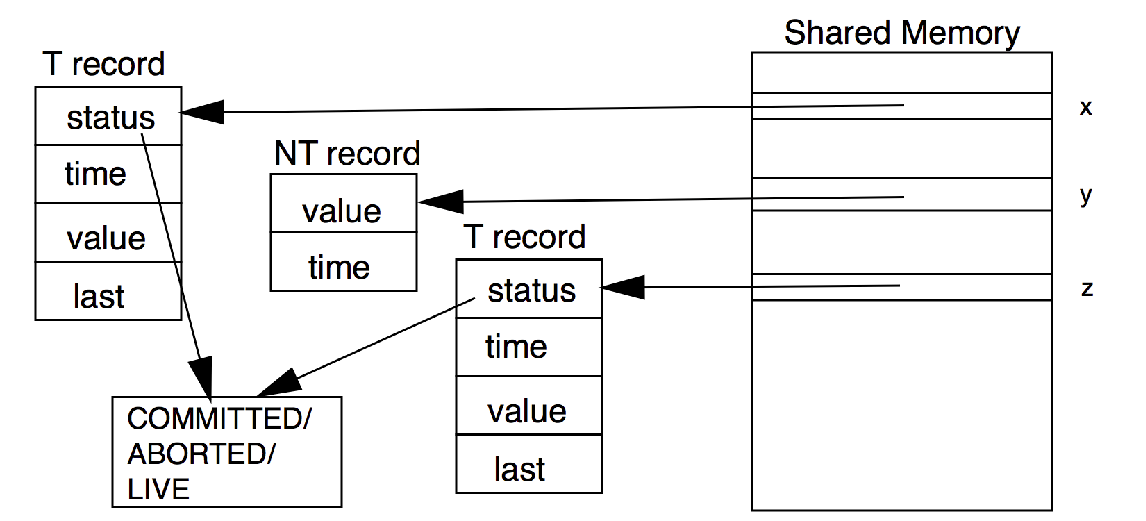
\includegraphics[width=0.6\textwidth]{SI/imgs/mem_setup_single}}
}
\caption{The memory set-up and the data structures that are used by the 
algorithm.}
\label{fig:mem_setup}
\end{figure*}

New T-records are created during the transactional write operations.
Then during
the commit operation the pointer stored at $\mathit{addr}$ is updated to point to this new T-record.
During NT-write operations new NT-records are created and the pointer at $\mathit{addr}$
is updated to point to the records.

When a read operation - be it transactional or non-transactional - accesses 
a shared variable it cannot know beforehand what type of record it will find. 
Therefore, it can be seen in the algorithm listings, that whenever 
a record is accessed, 
the operation checks its type, i.e., it checks 
whether it is a T-record or an NT-record (for example, line \ref{A02} in Fig.
\ref{fig:ntops} contains such a check. A T-record is {}``of type T'', while an 
NT-record is {}``of type NT''). 


\paragraph{T-record.}
A T-record is a structure containing the following fields.
\begin{description}
%\vspace{-0.1cm}
\item[$\mathit{status}$] This  field  indicates  the  state  of the  transaction  that  created  the
T-record. The  
state can either be LIVE, COMMITTED or ABORTED.
The state is initially set to LIVE and is not set to COMMITTED until during the commit operation when 
all locations of the transaction's write set have been set to point to the transaction's T-records
and the transaction has validated its read set.
Since a transaction can write to multiple locations, the $\mathit{status}$ field
does not directly store the state, instead it contains a
pointer to a memory location containing the state for the transaction.
Therefore the $\mathit{status}$ field of each T-record created by the same transaction will point to the same location.
This ensures that any change to the transaction's state is immediately recognized at each record.
%\vspace{-0.2cm}
\item[$\mathit{time}$] The  $\mathit{time}$  field of  a T-record  contains the  
value of  the $\mathit{GVC}$  at  the  moment the  record  was 
inserted to memory. %  into the  list of   records.
This is similar to the logical dates of TL2.
%\vspace{-0.2cm}
\item[$\mathit{value}$] This field contains the value that is meant to be written to the chosen 
memory location.
%\vspace{-0.2cm}
\item[$\mathit{last}$] During the commit operation, locations are updated to point
to the committing transaction's T-records, overwriting the previous value
that was stored in this location.
Failed validation or concurrent non-transactional operations may cause this transaction to abort 
after it updates some memory locations, but before
it fully commits.
Due to this, the previous value of the location needs to be available for future reads.
Instead of rolling back old memory values, the $\mathit{last}$ field of a T-record is used,
storing the previous value of this location.

\end{description}


\paragraph{NT-record.}
An NT-record is a structure containing the following fields.
\begin{description}
%\vspace{-0.1cm}
\item[$\mathit{value}$]
This field contains the value that is meant to be written to the chosen 
memory location.
%\vspace{-0.2cm}
\item[$\mathit{time}$]
As in the case of T-records, the $\mathit{time}$ field of NT-records 
also stores the value 
of the $\mathit{GVC}$ when the write took place.
%This field is 
%used to avoid inconsistencies %such as the ones illustrated by Figure 
%\ref{fig:timent}. 
%caused by the ABA problem.
\end{description}

Due to this different memory structure a shared lock array is no longer needed,
instead of locking each location in the write set during the commit operation, this algorithm
performs a compare and swap directly on each memory location changing the address to point to one of its T-records.
After a successful compare and swap
 and before the transactions status has been set to COMMITTED or ABORTED, the transaction effectively
owns the lock on this location.
Like in TL2, any concurrent transaction that reads the location and sees that it is locked ($\mathit{status} = $ LIVE) will
abort itself.

% During read operations (transactional or non-transactional) the additional data in these structures is used 
% to determine the most  recent valid value  of a variable.
% Should the item be of type NT-record,
% then it's $\mathit{value}$ field contains the most  
% recent valid value  of the variable. On the other hand,  should the item
%  be a  T-record, then if the $\mathit{status}$ field of
% the record is equal to COMMITTED,  
% the $\mathit{value}$ field represents the current value of the variable. Otherwise, the
% $\mathit{last}$ field contains the current value.

\paragraph{Transactional Read and Write Sets.}
Like TL2, read only transactions do not use read sets while update transactions do.
The read set is made up of a set of tuples for each location read, $\tuple{\mathit{addr, value}}$
where $\mathit{addr}$ is the address of the location read and $\mathit{value}$ is the value.
The write set is also made up of tuples for each location written by the transaction,
$\tuple{\mathit{addr, item}}$ where $\mathit{addr}$ is the location to be written
and $\mathit{item}$ is a T-record for this location.

\subsubsection{Discussion.}
One advantage of the TL2 algorithm is in its memory layout.
This is because reads and writes happen directly to memory (without indirection)
and the main amount of additional memory that is used is in the lock array.
Unfortunately this algorithm breaks that and requires an additional level of indirection
as well as additional memory per location.
While garbage collection will be required for old T- and NT-records, here we assume
automatic garbage collection such as that provided in Java, but additional solutions will be explored in future work.
These additional requirements can be an acceptable trade-off given that they are only
needed for memory that will be shared between transactions.
In the appendix of this paper we present two variations of the algorithm that trade
off different memory schemes for different costs to the transactional and
non-transactional operations.


%====================================================================

\subsection{Description of the Algorithm.}

The main goal of the algorithm is to provide strong isolation 
in such a way that  the non-transactional  operations are never blocked or aborted. 
In order  to achieve this,  the algorithm delegates most of its
concurrency   control   and  consistency   checks   to  the   transactional
code. Non-transactional  
operations access and modify  memory  locations without waiting for concurrent transactions
 and it is mainly up to transactions accessing the same location to
deal with ensuring safe concurrency.  As a
result, this algorithm gives high  priority   to non-transactional code. 

%=====================================================================
\subsection{Non-transactional Operations.}
Algorithm-specific  read  and write operations
shown in Fig. \ref{fig:ntops} must be used when a shared variable is accessed
accessed outside of a transaction.
As described in section \ref{sec:SIsolutions} this can be done by hand by the programmer,
but more appropriately a programmer will write normal shared reads and writes which will then
be automatically converted to non-transactional read (resp. write) operations by
the compiler or dynamically at runtime.

\begin{figure}[htb]
\centering{ \fbox{
\begin{minipage}[t]{1\linewidth}%{150mm}
%\footnotesize 
\scriptsize
\renewcommand{\baselinestretch}{2.5} 
%\resetline
%\setcounter{linecounter}{200}
\begin{tabbing}
aaaaaaa\=aa\=aaaaa\=aa\=aa\=\kill %~\\


{\bf operation}  ${\sf non\_transactional\_read}(\mathit{addr})$ {\bf is}\\
\line{A01} \> $\mathit{tmp} \gets (\downarrow \mathit{addr})$; \\ 
\line{A02} \> {\bf if} $( ~\mathit{tmp}$ is of type T $ \wedge (\downarrow \mathit{tmp.status}) \neq$ COMMITTED ) \\
%\line{A03}  \>\>  {\bf then if}  $(\mathit{tmp.time}  \leq \mathit{time}  \wedge  (\downarrow \mathit{tmp.status}) = $ LIVE) \\
\line{A03}  \>\>  {\bf then if}  $((\downarrow \mathit{tmp.status}) = $ LIVE) \\
\line{A04} \>\>\>\> {\bf then} \=${\sf \mathit{C\&S}}$($tmp.status$, LIVE, ABORTED) {\bf end if}; \\
%\line{A05} \>\> {\bf end if} \\
\line{A06} \>\>\> {\bf if} ($(\downarrow \mathit{tmp.status}) \neq $ COMMITTED)  \\
\line{A07} \>\>\>\> {\bf then} $\mathit{value} \gets \mathit{tmp.last}$ \\
\line{A08} \>\>\>\> {\bf else} $\mathit{value} \gets \mathit{tmp.value}$ \\
\line{A05} \>\>\> {\bf end if}; \\
\line{A09} \>\> {\bf else} $\mathit{value} \gets \mathit{tmp.value}$ \\
\line{A09A} \> {\bf end if}; \\
\line{A10} \> $\mathit{time} \gets {\sf max}(\mathit{time}, \mathit{tmp.time})$ \\
\line{A11} \> {\bf if} ($\mathit{time} = \infty$) {\bf then} $\mathit{time} = \mathit{GCV}$ {\bf end if}; \\
\line{A12} \> ${\sf return}$ ($\mathit{value}$) \\
{\bf end operation}. \\
\\
{\bf operation}  ${\sf non\_transactional\_write}(\mathit{addr, value})$ {\bf is}\\
\line{B01} \> allocate new variable $\mathit{next\_write}$ of type NT; \\
\line{B02} \> $\mathit{next\_write} \gets \mathit{(addr, value, \infty)}$; \\
\line{B03} \> $\mathit{addr} \gets (\uparrow \mathit{next\_write})$ \\
\line{B04} \> $\mathit{time} \gets \mathit{GVC}$; \\
\line{B05} \> $\mathit{next\_write.time} \gets \mathit{time}$; \\
{\bf end operation}.

\end{tabbing}
\normalsize
\end{minipage}
}
\caption{Non-transactional operations for reading and writing a variable.}
\label{fig:ntops}
}
\end{figure}

\paragraph{Non-transactional Read.}
The   operation  ${\sf   non\_transactional\_read()}$  is   used   to  read,
when not in a transaction, the value stored at
$\mathit{addr}$.
The  operation first  dereferences  the pointer  stored at  $\mathit{addr}$
(line \ref{A01}).
If the item is a T-record that was created by a 
transaction which  has not yet  committed then the $\mathit{value}$ field
cannot be immediately be read as the transaction might still abort.
% Also if the current process has read (or written to) a value that is more recent then the transaction
% (meaning the process's $\mathit{time}$ field is greater or equal to the T-records
% $\mathit{time}$, line \ref{A03}) then 
Then instead of waiting for the live transaction to finish committing it is directed to abort (line \ref{A04}),
ensuring that the operation's wait-free progress as well as opacity and strong isolation (containment specifically) is not violated.
From a T-record with a transaction that is not committed, the value from the $\mathit{last}$
field is stored to a local variable (line \ref{A07}) and will be returned on operation completion.
Otherwise the $\mathit{value}$ field of the T- or NT-record is used (line \ref{A08}).

% Once  the correct value  has been  found  and stored  in local  variable 
% $\mathit{value}$, the local $\mathit{time}$   
% variable  is updated  (lines \ref{A10}-\ref{A11}).  The updated  $\mathit{time}$
% value is used by non-transactional operations and is necessary in order to allow 
% the detection of consistency 
% violations such as the one illustrated by Figure \ref{fig:timent}. 
% By advancing the value of $\mathit{time}$ 
% through a non-transactional read operation, 
% the serialization order of this read operation with 
% respect to transactional or non-transactional operations 
% that it read from is reflected.

Next the process local variable $\mathit{time}$ is advanced to 
the maximal 
value among its current 
value and the logical date of the T- or NT-record whose value was read.
Finally if $\mathit{time}$ was set to $\infty$ on line \ref{A10}
(meaning the T- or NT-record had yet to set its $\mathit{time}$), then it is updated
to the $\mathit{GCV}$ on line \ref{A11}.
The updated  $\mathit{time}$
value is used 
%by non-transactional operations and is necessary 
to prevent consistency 
violations. %such as the one illustrated by Figure \ref{fig:timent}. 
%caused by the ABA problem.
Once these book-keeping 
operations are finished, the local variable $\mathit{value}$
is returned (line \ref{A12}).

\paragraph{Non-transactional Write.}
The operation ${\sf non\_transactional\_write()}$ is used to write to 
a shared variable $\mathit{var}$ 
by non-transactional code.
The operation takes as input the address of the shared variable as well as the 
value to be written to it.
This operation  
creates a  new  NT-record  (line  \ref{B01}),  fills  in  its  fields  (line
\ref{B02})  and 
changes the pointer stored in $\mathit{addr}$ so that it references the 
new record it has created  (line \ref{B03}).
Unlike update transactions, non-transactional writes do not increment
the global clock variable $\mathit{GCV}$.
Instead they just read $\mathit{GCV}$ and set the NT-record's time value as well as
the process local $\mathit{time}$ to the value read (line \ref{B04} and \ref{B05}).
Since the $\mathit{GCV}$ is not incremented, several NT-records might have the same
$\mathit{time}$ value as some transaction.
When such a situation is recognized where a live transaction has the same time value
as an NT-record the transaction must be aborted (if recognized during an NT-read operation,
line \ref{A04}) or perform read set validation (if during a transactional
read operation, line \ref{C05} of Fig. \ref{fig:tops}).
This is done in order to prevent consistency violations
caused by the NT-writes not updating the $\mathit{GCV}$. %such as the one shown in Figure \ref{fig:timent}.

%==================================================================
\subsection{Transactional Read and Write Operations.}

The transactional operations for performing reads and writes are 
presented in Fig. \ref{fig:tops}. 

\paragraph{Transactional Read.}

The operation ${\sf  transactional\_read()}$ takes $\mathit{addr}$ as
input. It starts by checking  
whether the  desired variable already  exists in the  transaction{}'s write
set, in which  
case  the   value  stored there  will   be  returned  (line
\ref{C01}). If the variable is not contained  
in  the write  set, the  pointer in  $\mathit{addr}$ is  dereferenced (line
\ref{C02}) and set to $\mathit{tmp}$. Once this is detected to be a T- or NT-record
some checks are then performed in order to ensure correctness.

In the case that $\mathit{tmp}$ is a T-record the operation must check to see
if the status of the transaction for this record is still LIVE and if it is
the current transaction is aborted (line \ref{C10}).
This is similar to a transaction in TL2 aborting itself when a locked location is found.
Next the T-record's $\mathit{time}$ field is checked, and (similar to TL2) if it 
greater then the process's local $\mathit{rv}$ value the transaction must abort 
(line \ref{C12}) in order to prevent consistency violations.
If this succeeds without aborting then the local variable $\mathit{value}$
is set depending on the stats of the transaction that created the T-record (line \ref{C10}-\ref{C11}).

In case $\mathit{tmp}$ is an 
NT-record (line \ref{C03}), the operation
checks whether the value of the $\mathit{time}$ field is
greater or equal to the process local $\mathit{rv}$ value.
If it is, then this write has possibly occurred after the start of this
transaction and there are several possibilities.
In the case of an update transaction validation must be preformed, ensuring
that none of the values it has read have been updated (line \ref{C05}).
In the case of a read only transaction, the transaction
is aborted and restarted as an update transaction (line \ref{C06}).
It is restarted as an update transaction so that it has a read set that it can validate
in case this situation occurs again.
Finally local variable $\mathit{value}$ is set to be the value
of the $\mathit{value}$ field of the $\mathit{tmp}$ (line \ref{C07}).

It should be noted that the reason why the checks are performed differently
for NT-records and T-records is because the NT-write operations do not
update the global clock value while update transaction do.
This means that the checks must be more conservative in order to ensure correctness.
If performing per value validation or restarting the transaction as an update transaction
is found to be too expensive, a third possibility would be to just increment the global
clock, then restart the transaction as normal.

Finally to finish the read operation, the $\tuple{\mathit{addr, value}}$
is added to the read set if the transaction is an update transaction (line \ref{C14}),
and the value of the local variable $\mathit{value}$  is returned.







\begin{figure} [htb]
\centering{ \fbox{
\begin{minipage}[t]{1\linewidth}%{150mm}
%\footnotesize 
\scriptsize
\renewcommand{\baselinestretch}{2.5} 
%\resetline
%\setcounter{linecounter}{200}
\begin{tabbing}
aaaaaaa\=aa\=aaaaa\=aa\=aa\=\kill %~\\


{\bf operation}  ${\sf transactional\_read}(\mathit{addr})$ {\bf is}\\
\line{C01} \> {\bf if} $\mathit{addr} \in \mathit{ws}$  {\bf then} ${\sf return}$ ($\mathit{item.value}$ from $\mathit{addr}$ in $\mathit{ws}$)  {\bf end if}; \\
\line{C02} \> $\mathit{tmp} \gets (\downarrow \mathit{addr})$; $\mathit{validate} \gets \sf{false}$;\\

\line{C03} \> {\bf if} ($\mathit{tmp}$ is of type NT)   \\
\line{C04} \>\> {\bf then} {\bf if} ($\mathit{tmp.time} \geq \mathit{rv}$) \bf{then} $\mathit{validate} \gets \sf{true}$ \bf{end if} \\
% % % % %\> \% Do validation to prevent abort due to a non-transactional write \\
% % % % \line{C05} \>\>\> {\bf then if} this is an update transaction {\bf then} add $\tuple{\mathit{addr,tmp.value}}$ to $\mathit{rs}$ and ${\sf validate\_by\_value}$(); \\
% % % % \line{C06} \>\>\>\>\> {\bf else} ${\sf abort}$() and restart as an update transaction {\bf end if}; \\
% % % % %\line{C14} \> {\bf if} this is an update transaction 
% % % % %                        {\bf then} add $\tuple{\mathit{addr,value}}$ to $\mathit{rs}$ {\bf end if}; \\
% % % % 
% % % % 
% % % % \line{C06A} \>\>\> {\bf end if}; \\
\line{C07} \>\>\> $\mathit{value} \gets \mathit{tmp.value}$; \\

\line{C08} \>\> {\bf else} \\
\line{C09} \>\>\> {\bf if} ($(\mathit{status} \gets (\downarrow \mathit{tmp.status})) \neq$ COMMITTED $)$ \\
\line{C10} \>\>\>\> {\bf then if} ($\mathit{status} =$ LIVE) {\bf then} ${\sf abort}()$  {\bf else} $\mathit{value} \gets \mathit{tmp.last}$ {\bf end if}; \\
\line{C11} \>\>\>\> {\bf else} $\mathit{value} \gets \mathit{tmp.value}$ \\
\line{C11A} \>\>\> {\bf end if}; \\
\line{C12} \>\>\> {\bf if} $(\mathit{tmp.time} > \mathit{rv})$ {\bf then} $\mathit{validate} \gets \sf{true}$ {\bf end if}; \\
% % % % \line{C14} \>\> {\bf if} this is an update transaction {\bf then} add $\tuple{\mathit{addr,value}}$ to $\mathit{rs}$ {\bf end if}; \\


\line{C13} \> {\bf end if}; \\

\line{C14} \> {\bf if} this is an update transaction
                        {\bf then} add $\tuple{\mathit{addr,value}}$ to $\mathit{rs}$ {\bf end if}; \\

\line{C14A} \> {\bf if} ($\mathit{validate}$) \\
\line{C14B} \>\> {\bf then if} this is an update transaction {\bf then if} (${\sf validate\_by\_value}$()) {\bf then} $\sf{abort}()$ {\bf end if}; \\
\line{C14C} \>\>\>\> {\bf else} ${\sf abort}$() and restart as an update transaction {\bf end if}; \\


\line{C14D} \> {\bf end if}; \\


\line{C15} \> ${\sf return}$ ($\mathit{value}$) \\
{\bf end operation}. \\
\\
{\bf operation}  ${\sf transactional\_write}(\mathit{addr, value})$ {\bf is}\\
\line{D01} \> {\bf if} $\mathit{addr} \not\in \mathit{ws}$  \\
\line{D02} \>\> {\bf then} \> allocate a new variable $item$ of type $T$; \\
\line{D03} \>\>\> $\mathit{item}  \gets (\mathit{value, (\uparrow status), \infty})$; 
                   $\mathit{ws} \gets \mathit{ws} \cup \tuple{\mathit{addr, item}}$; \\
\line{D04} \>\> {\bf else} \> set $\mathit{item.value}$ with $\mathit{addr}$ in $\mathit{ws}$ to $\mathit{value}$ \\
\line{D05} \> {\bf end if}; \\
{\bf end operation}.
\end{tabbing}
\normalsize
\end{minipage}
}
\caption{Transactional operations for reading and writing a variable.}
\label{fig:tops}
}
\end{figure}

\paragraph{Transactional Write.}
The ${\sf transactional\_write()}$ operation
takes $\mathit{addr}$ as input value, as well as the value 
to be written to $\mathit{var}$. As  TL2, the algorithm 
performs commit-time updates of the variables it writes to. 
For this reason, the transactional write  
operation simply creates a T-record and fills in some of its 
fields (lines \ref{D02} - \ref{D03}) and 
adds it to the write set.
However, in the case that a T-record corresponding to $\mathit{addr}$  was
already present in  the write set, the
$\mathit{value}$ field of the corresponding  
T-record is simply updated (line \ref{D04}).


\paragraph{Begin and End of a Transaction} 
The operations that begin and end a transaction are ${\sf begin\_transaction()}$ 
and ${\sf try\_to\_commit()}$, presented in Fig. \ref{fig:tbc}. 
%Operation ${\sf begin\_transaction()}$ 
%initializes local variables that will be necessary 
%for the execution of the transaction.
Local variables necessary for transaction execution are initialized by  ${\sf begin\_transaction()}$.
This includes $\mathit{rv}$
which is set to $\mathit{GCV}$ and, like in TL2, is used during transactional
reads to ensure correctness, 
as well as $\mathit{status}$ which is set to LIVE and the read and write sets
which are initialized as empty sets.
(lines \ref{START1}-\ref{START3}). 

\begin{figure} [htb]
\centering{ \fbox{
\begin{minipage}[t]{1\linewidth}%{150mm}
%\footnotesize 
\scriptsize
\renewcommand{\baselinestretch}{2.5} 
%\resetline
%\setcounter{linecounter}{200}
\begin{tabbing}
aaaaaaa\=aa\=aaaaa\=aa\=aa\=\kill %~\\

{\bf operation}  ${\sf begin\_transaction}()$ {\bf is}\\
\line{START1} \> determine whether transaction is update transaction based on compiler/user input \\
\line{START2} \> $\mathit{rv} \gets \mathit{GVC}$; 
                 Allocate new variable $\mathit{status}$; \\
\line{START3} \> $\mathit{status} \gets $LIVE; \ $\mathit{ws} \gets \emptyset$; $\mathit{rs} \gets \emptyset$ \\
%\line{DA03} \> more??? \\
{\bf end operation}. \\
\\
{\bf operation}  ${\sf try\_to\_commit}()$ {\bf is}\\
\line{DA01} \> {\bf if} $(\mathit{ws} = \emptyset)$ {\bf then} ${\sf return}$ (COMMITTED) {\bf end if}; \\

% \line{DA01a} \> $\mathit{abort} \gets \lit{false}$; \\

\line{DA02} \> 
{\bf for each} $(\tuple{\mathit{addr, item}} \in \mathit{ws})$ {\bf do} \\

\line{DA03} \>\> $\mathit{tmp} \gets (\downarrow \mathit{addr})$; \\


\line{DA04} \>\> {\bf if} 
   ($\mathit{tmp}$ is of type $T \wedge (\mathit{status} \gets (\downarrow \mathit{tmp.status})) \neq$ COMMITTED $)$  \\
\line{DA05} \>\>\> {\bf then if} ($\mathit{status} =$ LIVE) {\bf then} $\sf{abort}()$  {\bf else} $\mathit{item.last} \gets \mathit{tmp.last}$ {\bf end if}; \\
\line{DA06} \>\>\> {\bf else} $\mathit{item.last} \gets \mathit{tmp.value}$ \\
\line{DA06A} \>\> {\bf end if}; \\

\line{DA07} \>\> $\mathit{item.time} \gets \mathit{tmp.time}$; \\
\line{DA07a} \>\> {\bf if} ($\mathit{item.time} = \infty$) {\bf then} $\mathit{item.time} \gets \mathit{GCV}$ {\bf end if}; \\

\line{DA08} \>\> {\bf if} $(\neg {\sf \mathit{C\&S}}(\mathit{addr, tmp, item}))$ {\bf then} $\sf{abort}()$ {\bf end if}; \\
%\line{DA09} \>\>\> {\bf then} ${\sf abort}()$ \\
%\line{DA10} \>\> {\bf end if} \\

\line{DA11} \> {\bf end for}; \\

\line{DA12} \> $\mathit{time} \gets {\sf increment\&fetch}(\mathit{GVC})$; \bf{if} (${\sf validate\_by\_value}()$) {\bf then} $\sf{abort}()$ {\bf end if}; \\

%\line{DA13} \> ${\sf validate\_by\_value}()$;  \\


%\> \% Ensure the writes haven't been overwritten by non-transactional writes \\

\line{DA14} \> 
{\bf for each} ($\tuple{\mathit{addr, item}} \in \mathit{ws}$) {\bf do} \\
\line{DA15} \>\> $\mathit{item.time} \gets \mathit{time}$; \\
\line{DA16} \>\> {\bf if} $(\mathit{item} \neq (\downarrow \mathit{addr}))$  
                 {\bf then}  
		    $\sf{abort}()$
                {\bf end if}; \\

\line{DA17} \> {\bf end for}; \\
% \line{DA17a} \> {\bf if} $\mathit{abort}$ {\bf then} ${\sf abort}()$ {\bf end if}; \\
\line{DA18} \> {\bf if} ${\sf \mathit{C\&S}}$($\mathit{status}$, LIVE, COMMITTED) \\
\line{DA19} \>\> {\bf then} \> ${\sf return}$ (COMMITTED)\\
\line{DA20} \> \> {\bf else} \= ${\sf abort}()$ \\
\line{DA21} \> {\bf end if};  \\
{\bf end operation}.

\end{tabbing}
\normalsize
\end{minipage}
}
\caption{Transaction begin/commit.}
\label{fig:tbc}
}
\end{figure}

After  performing all  required read  and write  operations,  a transaction
tries to commit, using the operation  ${\sf try\_to\_commit()}$.
Similar to TL2, a ${\sf try\_to\_commit()}$ operation 
starts by trivially committing if the transaction was a read-only one 
(line \ref{DA01}) while
an update transaction must announce to concurrent operations what locations it will be updating
(the items in the write set).
However, the algorithm  differs 
here from TL2, given that 
it is faced with concurrent non-transactional operations
that do not rely on locks and never block. 
This implies 
that even after acquiring the locks for all items in its write set, 
a transaction could be {}``outrun'' by 
a non-transactional operation that writes to one of those items
causing the transaction to be required to abort in order to ensure correctness. 
As described previously, while TL2 locks items in its write set using a
lock array, this algorithm compare and swaps pointers directly to the T-records
in its write set (lines \ref{DA02}-\ref{DA11}) while keeping a reference to the previous value.
The previous value is stored in the T-record before the compare and swap is performed (lines \ref{DA05}-\ref{DA06})
with a failed compare and swap resulting in the abort of the transaction.
If while performing these compare and swaps the transaction notices
that another LIVE transaction is updating this memory, it aborts itself
(line \ref{DA05}).
By using these T-records instead of locks concurrent operations have access to necessary metadata
used to ensure correctness.

The operation then advances the $\mathit{GVC}$, taking the
new value of the clock as the logical time for this transaction (line \ref{DA12}).
Following this, the read set of the transaction is validated for
correctness  (line \ref{DA12}). %was: (line \ref{DA13}).
Once validation has been performed the operation must
ensure that non of its writes have been concurrently
overwritten by non-transactional operations (lines \ref{DA14}-\ref{DA17})
if so then the transaction must abort in order to (line \ref{DA16}) to ensure consistency.
During this check the transaction updates the $\mathit{time}$
value of its T-records to the transactions logical time (line \ref{DA15})
similar to the way TL2 stores time values in the lock array
so that future operations will know the serialization of this transaction's updates.

Finally the
transaction can mark its updates as valid by 
changing its 
$\mathit{status}$ variable from LIVE to COMMITTED (line \ref{DA18}).
This is done using a compare and swap as there could be
a concurrent non-transactional operations trying to abort the transaction.  
If this succeeds then the transaction has successfully committed, otherwise
it must abort and restart.


\begin{figure} [htb]
\centering{ \fbox{
\begin{minipage}[t]{1\linewidth}%{150mm}
%\footnotesize 
\scriptsize
\renewcommand{\baselinestretch}{2.5} 
%\resetline
%\setcounter{linecounter}{200}
\begin{tabbing}
aaaaaaa\=aa\=aaaaa\=aa\=aa\=\kill %~\\

{\bf operation} ${\sf validate\_by\_value}()$ {\bf is}\\
\line{H01} \> $\mathit{rv} \gets \mathit{GVC}$; \\
\line{H02} \> {\bf for each} $\tuple{\mathit{addr, value}}$ in $\mathit{rs}$ {\bf do} \\
\line{H03} \>\> $\mathit{tmp} \gets (\downarrow \mathit{addr})$; \\
\line{H04} \>\> {\bf if} ($\mathit{tmp}$ is of type T $ \wedge \mathit{tmp.status} \neq $ COMMITTED) \\
\line{H05} \>\>\> {\bf then if} ($\mathit{tmp.status} =$ LIVE $\wedge \mathit{item} \not \in \mathit{ws}$)
     {\bf then} $\sf{return}(\sf{true})$ {\bf end if}; \\
\line{H06} \>\>\>\> $\mathit{new\_value} \gets \mathit{tmp.last}$; \\
\line{H07} \>\>\> {\bf else} $\mathit{new\_value} \gets \mathit{tmp.value}$ \\
\line{H07A} \>\> {\bf end if}; \\
\line{H08} \>\> {\bf if} ($\mathit{new\_value} \neq \mathit{value}$)
     {\bf then} $\sf{return}(\sf{true})$ {\bf end if}; \\
\line{H09} \> {\bf end for}; \\
\line{H10} \> $\sf{return}(\sf{false})$. \\
{\bf end operation}. \\
\\
{\bf operation} ${\sf abort}()$ {\bf is}\\
\line{AB01} \> $\mathit{status} \gets $ ABORTED; \\
\line{AB02} \> the transaction is aborted and restarted \\
%\line{H21} \> free items in $\mathit{ws}$, $\mathit{rs}$, and $\mathit{ntrs}$; \\
%\line{H22} \> jump to line \ref{START1} \\
{\bf end operation}. \\
\end{tabbing}
\normalsize
\end{minipage}
}
\caption{Transactional helper operations.}
\label{fig:helpers}
}
\end{figure}


\paragraph{Transactional Helping Operations.} 
Apart from the basic operations for starting, committing, 
reading and writing, a transaction makes use of helper 
operations to perform aborts and validate the read set.
 Pseudo-code for this kind of helper operations 
is given in Fig. \ref{fig:helpers}.

Operation ${\sf validate\_by\_value()}$ is an operation that performs 
validation of the read set of a transaction. 
Validation fails 
if any location in $\mathit{rs}$ is 
currently being updated by another transaction (i.e. $\mathit{tmp.status} = $ LIVE) (line \ref{H05})
or has had its changed since it was first read by the transaction (line \ref{H08})
otherwise it succeeds.
The transaction is directed to abort if validation fails (lines \ref{H05}, \ref{H08}) by returning $\sf{true}$,
returning $\sf{false}$ otherwise.
Note that in the case that a location is being updated ($\mathit{tmp.status} = $ LIVE) and the location
is in the write set of the current transaction then it does not abort, as this record belongs to the transaction
currently being executed by the process performing the validation.
Instead the $\mathit{last}$ value of the record is validated.
Before the validation is performed the local variable $\mathit{rv}$ is updated
to be the current value of $\mathit{GVC}$ (line \ref{H01}).
This is done because if validation succeeds then transaction is valid at this time
with a larger
clock value possibly preventing future validations and aborts.

When a transaction is aborted in the present algorithm, 
the status of the current transaction is set to ABORTED (line \ref{AB01}) and
it is immediately restarted as a new transaction.

%========================================================================




\section{Proof of correctness}
This section will prove the correctness of the algorithm by showing the linearizability
of the transactions and non-transactional operations.
Specifically we will show that every transaction (aborted or committed) as well
as non-transactional operations have a unique linearization point, meaning that
there is some instant in time during the execution of each operation where it
appears to have taken place.
Note that we do not use an STM specific consistency criterion
such as opacity or virtual world consistency to prove correctness as they do not consider
non-transactional operations.

Before detailing the linearization points of the operations we will introduce a few lemmas that will help
with the proofs.

\begin{lemma}
\label{lemma:si-nochange}
Neither the $\mathit{value}$ field of a T or NT record nor the $\ms{last}$ field of a T record is changed once a pointer in shared memory is set to 
reference the record.
\end{lemma}
\begin{proof}
In the case of an NT record, the $\mathit{value}$ field is set just once on line \ref{B02} of $\sf{non\_transactional\_write}$,
which is just after the record is allocated, and before any shared pointers are set.
For a T record, allocation happens on line \ref{D02} of $\sf{transactional\_write}$,
then the $\mathit{value}$ field is set on lines \ref{D03} and \ref{D04} of the same operation.
The $\mathit{last}$ field is set later, but just once on line \ref{DA05} or \ref{DA06} of the $\sf{try\_to\_commit}$ operation
and the record is not referenced by a shared pointer until later in this operation
by performing a compare and swap on line \ref{DA08}.
\end{proof}


\begin{lemma}
\label{lemma:si-statusonce}
The $\ms{status}$ field of a transaction record will change from LIVE to either COMMITTED or ABORTED
exactly once.
\end{lemma}
\begin{proof}
The operation $\sf{begin\_transaction}$ is called each time a new transaction start and each time a transaction is aborted.
During this operation a new $\mathit{status}$ variable is allocated and is set to LIVE.
The status variable is then accessible by the process that is executing the transaction or through T records created during the
transaction (line \ref{D03} of $\sf{transaction\_write}$).
$\mathit{status}$ can be modified in three places:
On line \ref{A04} of $\sf{non\_transactional\_read}$ and on line \ref{DA18} of $\sf{try\_to\_commit}$, but in both these cases
the value of $\mathit{status}$ is changed from LIVE to either COMMITTED or ABORTED by a compare and swap.
The third place is on line \ref{AB01} of the $\sf{abort}$ where $\mathit{status}$ is set to ABORTED by a normal write, but
here $\mathit{status}$ must either still be LIVE, or already ABORTED because if the compare and swap from LIVE to COMMITTED was
successful then the transaction is guaranteed to be completed (lines \ref{DA18}--\ref{DA20} of $\sf{try\_to\_commit}$).
\end{proof}


\begin{lemma}
\label{lemma:si-samevalue}
For any T or NT record that is referenced by $\mathit{addr}$, any read operation (transactional or non-transactional) or validation (from $\sf{validate\_by\_value}$) to
$\mathit{addr}$ that dereferences this record will return (or validate) the same value.
\end{lemma}
\begin{proof}
There are two cases to consider, when the record dereferenced is of type NT and when the record is of type T.
\paragraph{NT Record} In this case using lemma \ref{lemma:si-nochange} and the looking at the code it is easy to see that both the transactional and non-transactional read
as well as validation operations
return/validate the value contained in the $\ms{value}$ field of the NT record dereferenced.
In the case where a $\sf{transaction\_read}$ causes a transactional abort, even though $\mathit{value}$ is not returned, linearizability is not violated
as aborted transactions appear to have not executed at all.
\paragraph{T Record} This case is a bit more difficult as the value returned depends on the $\mathit{status}$ of the transaction
that created this record.
First consider any $\sf{non\_transaction\_read}$ that has dereferenced this object, on line \ref{A04} the compare and swap ensures that the status of the transaction is
no longer LIVE.
Now by lemma \ref{lemma:si-statusonce} we know that $\mathit{status}$ will only change from LIVE once.
So if $\mathit{status}$ is ABORTED then the $\ms{last}$ field is returned, otherwise if COMMITTED then the $\mathit{value}$ field is returned.
Next consider any $\sf{transaction\_read}$ that dereferences this object, like with the NT reads,
(and using lemma \ref{lemma:si-statusonce}) if
$\mathit{status}$ is ABORTED then the $\ms{last}$ field is returned and if COMMITTED then the $\mathit{value}$ field is returned.
Otherwise in the case that $\mathit{status}$ is still LIVE, the transaction simply aborts (line \ref{C10}).
The $\sf{validate\_by\_value}$ operation follows the same pattern, with the exception if the $\mathit{status}$ is LIVE and
is in the write set of the current transaction.
In this case the process executing the validation is also the one who owns the record being validated, but here the compare
and swap on line \ref{DA08} of $\sf{try\_to\_commit}$ ensures that the value previously at this location is now in the $\mathit{last}$
field of this record.
\end{proof}




\begin{lemma}
\label{lemma:si-ntwrite}
The $\sf{non\_transactional\_write}$ operation is linearizable.
\end{lemma}
\begin{proof}
The linearization point of the $\sf{non\_transactional\_write}(addr,value)$ operation
is line \ref{B03} where the value of $\mathit{addr}$ is set to point to $\sf{next\_write}$.
There is no pre-condition needed for this operation as it acts as a simple write operation.
The post-condition is that the value in memory at $\mathit{addr}$ is $\mathit{value}$, meaning that $\mathit{next\_write.value}$ is returned by 
read operations to $\mathit{addr}$ (transactional and non-transactional) that are linearized after the write.
For either type of read operation their linearization point is when $\mathit{addr}$ is accessed (as will be detailed in further lemmas),
therefore any read operation linearized after this NT-write (and before another operation modifies $\mathit{addr}$)
will dereference the pointer written by the NT-write.
Lemma \ref{lemma:si-samevalue} completes the proof.
\end{proof}


\begin{lemma}
\label{lemma:si-ntread}
The $\sf{non\_transaction\_read}$ operation is linearizable.
\end{lemma}
\begin{proof}
The linearization point of the $\sf{non\_transaction\_read}(addr, value)$ is line \ref{A01} where the record
pointed to by $\mathit{addr}$ is dereferenced from memory.
The pre and post conditions are that the value in memory at $\mathit{addr}$ is $\mathit{value}$, or more specifically, 
any other read operation to $\mathit{addr}$ (transactional and non-transactional) whose access to $\mathit{addr}$
(line \ref{A01} of $\sf{non\_transaction\_read}$ and \ref{C01} of $\sf{transaction\_read}$) dereferences
the same record as $\mathit{tmp}$ returns the same value.
Since the object dereferenced at the linearization point is pointed to by $\mathit{addr}$ then the proof follows from
lemma \ref{lemma:si-samevalue}.
\end{proof}



\begin{lemma}
\label{lemma:si-rvvalid}
The value validated or returned by a successful $\sf{transactional\_read}$ operation to $\mathit{addr}$ is the same
value that would be validated or returned by a read (non-transactional or transactional) at the time the most recent
$\mathit{rv}$ was set for this transaction.
\end{lemma}
\begin{proof}
By lemma \ref{lemma:si-samevalue} we know that for any record dereferenced the value read or validated will
always be the same for that record, so the rest of this proof will consider that value when discussing
a dereferenced record.
There are two places where $\ms{rv}$ can be set, either at the start of a transaction on line \ref{START2} of the
$\sf{begin\_transaction}$ operation, or before validation on line \ref{H01} the $\sf{validate\_by\_value}$ operation.


For the $\sf{validate\_by\_value}$ case we know that every location read so far by the transaction is contained
in the read set (including the current location) before $\mathit{rv}$ is set.
After $\mathit{rv}$ is set, every location in the read set is validated, ensuring that each location contains the same
value as when it was previously read.
From this it is easy to see that when $\mathit{rv}$ is set, none of the values have been changed.

Let us now consider the case where the most recent value for $\ms{rv}$ was most recently set in $\sf{begin\_transaction}$.

\paragraph{T record} If the object dereferenced on line \ref{C01} of $\sf{transactional\_read}()$ is an NT record then we must have $\mathit{tmp.time} < \mathit{rv}$
as otherwise a validation would have been called, updating $\mathit{rv}$.
On line \ref{B03} of $\sf{non\_transactional\_write}$ operation $\mathit{addr}$ is set to reference the NT record, following this
$\mathit{GCV}$ is read which is then used to update the record's $\mathit{time}$ field.
Now, as previously stated this value must be smaller then $\mathit{rv}$, and given that the value of $\mathit{rv}$
was set using $\mathit{GCV}$, which is a synchronized growing counter, $\mathit{addr}$ must have been set to reference
this NT record before $\mathit{rv}$ was set, and has not changed up to the point where the record was dereferenced by the read.

\paragraph{T record} If the object dereferenced on line \ref{C01} of $\sf{transactional\_read}()$ is a T record then we must have $\mathit{tmp.time} \leq \mathit{rv}$ and 
$\mathit{tmp.status} = $ COMMITTED or $\mathit{tmp.status} = $ ABORTED, otherwise the transaction would have aborted.
Given this, we just need to show that the T record dereferenced was in memory before $\mathit{GCV}$ was incremented to the value
read in $\sf{begin\_transaction}$ (i.e. before $\mathit{GCV} = \mathit{rv}$).
First consider the case where $\mathit{tmp.status} = $ COMMITTED, given that $\mathit{tmp}$ is a T record, it was created
during a $\sf{try\_to\_commit}$ operation.
On line \ref{DA08} the compare and swap ensures that $\mathit{tmp}$ is referenced to by $\mathit{addr}$ before the transaction
increases $\mathit{GCV}$ by performing an increment and fetch.
Then on line \ref{DA15}, the value returned from the increment and fetch is used to set the $\mathit{time}$ field of each T record
created by the transaction.
Given this and that we know $\mathit{tmp.time} \leq \mathit{rv}$, $\mathit{tmp}$ must have been referenced by $\mathit{addr}$ before
$\mathit{GCV} = \mathit{rv}$.
Now consider the case where $\mathit{tmp.status} = $ ABORTED, the compare and swap on line \ref{DA08} of $\sf{try\_to\_commit}$ ensures
that the value in $\ms{tmp.last}$ was the previous value at $\ms{addr}$ as well as $\mathit{tmp}$ is referenced to by $\mathit{addr}$
before the increment and fetch.
Following this, like in the case where $\mathit{tmp.status} = $ COMMITTED we have the value returned from the increment and fetch
used to set the $\mathit{time}$ field of each T record created by the transaction.
Resulting in the fact that $\mathit{tmp}$ must have been referenced by $\mathit{addr}$ before $\mathit{GCV} = \mathit{rv}$.

Finally given that $\sf{begin\_transaction}$ is called only once per transaction and is performed before any read or validation is performed,
all the values returned by reads were the same when $\mathit{rv}$ was set.
\end{proof}




\begin{lemma}
\label{lemma:si-tread}
A successful $\sf{transaction\_read}$ operation (i.e. one that does not cause the transaction to abort) in linearizable,
at a point that includes it as well all previous reads of the transaction.
\end{lemma}
\begin{proof}
For the $\sf{transaction\_read}$ operation the linearization point is the most recent time that $\mathit{rv}$ was set for the transaction.
This could have been 
The pre and post conditions are that the values returned by this and all the previous reads of the transaction are the values in memory, or more specifically, 
(using lemma \ref{lemma:si-samevalue}) at the linearization point for each $\mathit{addr}$ read (including the current one) the location points to the record
that contains the same value that was read.
The proof of this lemma follows directly from lemma \ref{lemma:si-rvvalid}.
% We must consider whether the type of record that is dereferenced on line \ref{} is an NT or T record.
% \paragraph{NT record}
% For the NT-record we have two cases depending on the value read from $\mathit{tmp.time}$.
% \begin{itemize}
% \item \bf{$\mathit{tmp.time} \geq \mathit{rv}$}
% Here the linearization point is on line \ref{}, just before the call to $\sf{validate\_by\_value}$.
% Using lemma \ref{lemma:si-samevalue} and the fact that this operation validates each value in the read set,
% aborting if any change is found, it is easy to see that the pre and post conditions are satisfied.
% \item \bf{$\mathit{tmp.time} < \mathit{rv}$}
% In this case the linearization point was the time that the value of $\mathit{rv}$ was set.
% \end{itemize}
% \paragraph{T record}
\end{proof}


\begin{lemma}
\label{lemma:si-abort}
An aborted transaction makes no changes to the state of memory.
\end{lemma}
\begin{proof}
For this proof we only need to consider transactions that abort after they have performed
at least one successful compare and swap on line \ref{DA08} of $\sf{try\_to\_commit}$ as transactions
that have aborted before this have not made any modifications to shared memory.
On line \ref{DA08} the transaction compares and swaps each of its T records from its write set to
shared memory.
What is important here is that before the compare and swap the transaction updates the $\ms{last}$
field of the T record for $\mathit{addr}$ using either the $\mathit{value}$ or the $\mathit{last}$ field of the current
record at $\mathit{addr}$.
The $\mathit{value}$ field is used if the record is of type NT or comes from a committed transaction, otherwise the $\mathit{last}$
field is used, this follows the same pattern as the read and validate operations which were shown to all pick the same value
from a record in lemma \ref{lemma:si-samevalue}.
Now by using a compare and swap on line \ref{DA08} when adding the T record to memory, we ensure that the record in memory has not
changed since the $\mathit{last}$ field of the new record was set.
Now given that the transaction will abort (setting its $\mathit{status}$ to aborted), any read or validation that dereferences
this record will use the $\mathit{last}$ field which is the same value that was in memory previously.
\end{proof}



\begin{lemma}
\label{lemma:si-commit}
A committed transaction is linearizable.
\end{lemma}
\begin{proof}
For the precondition of the committed transaction we have the requirement
that for each of the locations in the transaction's read set that the value
contained in the record referenced by the address is equal to the value 
previously read by the transaction.
The post condition is that for each of the locations in the transaction's write set
that the value written by the transaction is the one contained in the record
referenced by the address in memory.
Here the linearization point is line \ref{DA12}, just after the transactions T records
have been pointed to by performing compare and swaps, and before the call to
$\sf{validate\_by\_value}$.
The precondition is ensured by the subsequent call to $\sf{validate\_by\_value}$,
as if any location in the read set has been changed since it was first read then
the transaction would abort.
The post condition is ensured by the for loop on lines \ref{DA15}-\ref{DA17} as well
as the compare and swap on line \ref{DA18} changing the transaction's $\mathit{status}$
from LIVE to COMMITTED.
The for loop checks the $\mathit{addr}$ for each record in the write set seeing
if there has been a more recent write updating this location, aborting the transaction
if there is.
Finally the compare and swap setting $\mathit{status}$ to COMMITTED ensures
that any future read (transactional or non-transactional) that dereferences one of
the records in the transaction's write set returns the value written by the transaction.
Lemma \ref{lemma:si-samevalue} ensures that any read or validation to any one of these
records returns the same value.
It is interesting to note that at the linearization point the transaction is not
guaranteed to commit, but lemmas \ref{lemma:si-abort} and \ref{lemma:si-samevalue}
ensure that in the case the transaction does abort, it still appears to have not happened
at all.
The reason for this is to ensure the progress of non-transactional operations they might
need to abort a transaction in the process of committing in order to ensure correctness.
\end{proof}



\begin{theorem}
\label{theorem:si-lin}
The algorithm provides linearizability for both committed and aborted transactions
and non-transactional reads and writes.
\end{theorem}
\begin{proof}
This follows directly from lemmas \ref{lemma:si-ntwrite}, \ref{lemma:si-ntread}, \ref{lemma:si-tread},
and \ref{lemma:si-commit}.
\end{proof}



\begin{figure} [htb]
\centering{ \fbox{
\begin{minipage}[t]{1\linewidth}%{150mm}
%\footnotesize 
\scriptsize
\renewcommand{\baselinestretch}{2.5} 
%\resetline
%\setcounter{linecounter}{200}
\begin{tabbing}
aaaaaaa\=aa\=aaaaa\=aa\=aa\=\kill %~\\


\line{A03a}  \>  {\bf then if}  $(\mathit{tmp.time}  \leq \mathit{time}  \wedge  (\downarrow \mathit{tmp.status}) = $ LIVE) \\

\end{tabbing}
\normalsize
\end{minipage}
}
\caption{Modified line of the NT-read operation.}
\label{fig:ser}
}
\end{figure}





\section{From linearizability to serializability}

In algorithm \ref{fig:ntops} whenever a NT-read operation encounters
a transaction in the process of committing it immediately attempts to abort the transaction.
Interestingly this can be prevented
in the case that the thread performing the NT-read has not observed a write that is serialized after the transaction
by serializing the NT-read before the transaction.
Algorithm \ref{fig:ser} describes the changes to the NT-read operation, line \ref{A03} of
the original algorithm is modified to become line \ref{A03a} in algorithm \ref{fig:ser}.
It is important to note that this change means that the NT-reads will no longer be linearizable,
instead they become serializable.
The reason for this is that the NT-read operation could have started after the linearization point
of a transaction, but before the transaction the transaction's status has been changed from LIVE to
COMMITTED.
Then if the NT-read returns the value contained in $\mathit{tmp.last}$ its real time occurrence was
after the linearization point of the transaction, but it is serialized before the transaction.









%\section{Refernces}\label{references}

% \begin{thebibliography}{4}

% \bibitem{afek10}
%  Afek, Y.,  Avni, H.,   Dice, D.,  Shavit, N.: Efficient lock free privatization. 
% In: {\it Proc.  14th Int'l conference on Principles of Distributed Systems 
% (OPODIS'10)}, pp. 333--347, Springer-Verlag,  LNCS \#6490 (2010) 
% 
% \bibitem{CIR12} 
% Crain, T., Imbs, D.,  Raynal, M.: 
% Towards a Universal Construction for Transaction-based Multiprocess Programs.
% In: {\it Proc. 13th Int'l Conference on Distributed Computing and Networking (ICDCN'12)}, 
% pp. 61--75, Springer Verlag LNCS \#7129 (2012) 
% 
% \bibitem{DS09}
% Dalessandro, L., Scott, M.:
% Strong Isolation is a Weak Idea. 
% In: {\it Proc. Workshop on transactional memory (TRANSACT'09)} (2009)
% 
% \bibitem{dice10}
% Dice, D., Matveev, A.,  Shavit, N.:
% Implicit privatization using private transactions. 
% In: {\it Proc. Workshop on transactional memory (TRANSACT'10)} (2010)
% 
% \bibitem{dice06}
% Dice, D., Shalev O., Shavit, N.:
% Transactional Locking II.
% In: {\em Proc. 20th Int'l Symp. on Distributed Computing (DISC'06)},
% Springer-Verlag, LNCS \#4167, pp.~194--208 (2006)
% 
% \bibitem{guerraoui08}
% Guerraoui, R., Kapalka, M.:  On the correctness of transactional memory. 
% In: {\it  Proc. 13th ACM SIGPLAN Symposium on Principles and Practice of 
% Parallel Programming (PPoPP '08)},  ACM Press, pp.  175--184 (2008)
% 
% \bibitem{harris06}
%  Harris, T.,  Larus, J.,  Rajwar, R.:
% Transactional Memory, 
% {\it 2nd edition, Synthesis Lectures on Computer Architecture},
% Morgan \& Claypool Publishers (2006)
% 
% \bibitem{herlihy93}
% Herlihy, M., Moss J.M.B.: Transactional memory: architectural support for lock-free data structures, 
% In: {\it Proc.  of the 20th annual Int'l Symposium on Computer Architecture 
% (ISCA '93)}, ACM Press, pp. 289--300 (1993)
% 
% \bibitem{IR09} 
% Imbs, D., Raynal, M.: 
% A versatile   STM protocol with invisible read operations 
% that satisfies  the  virtual world consistency condition.
% In: {\it   16th  Colloquium   on  Structural   Information   and  Communication Complexity  (SIROCCO'09)}, 
% Springer Verlag LNCS   \#5869, pp. 266--280 (2009)
% 
% \bibitem{ma07}
%  Maessen, J.-W., Arvind, M.:
%  Store Atomicity for Transactional Memory. 
% {\it Electronic  Notes  on Theoretical  Computer Science}, 
% 174(9):117--137 (2007).
% 
% \bibitem{blundell06}
%  Martin, M.,  Blundell, C., Lewis, E.:
%  Subtleties of Transactional Memory Atomicity Semantics. 
% {\it IEEE Computer Architecture  Letters},  5(2):  (2006)
% 
% \bibitem{MS12}
% Matveev, A.,  Shavit, N.:
% Towards a Fully Pessimistic STM Model. 
% In: {\it Proc. Workshop on transactional memory (TRANSACT'12)} (2012)
% 
% \bibitem{MTCM07}
% Minh, C., Trautmann, M., Chung, J., McDonald, A., Bronson, N., Casper, J., Kozyrakis, C., Olukotun, K.:
% An effective hybrid transactional memory system with strong isolation guarantees.
% In: {\it SIGARCH Comput. Archit. News}, 35(2):69--80 (2007)
% 
% \bibitem{P79}
% Papadimitriou, Ch.H.:
% The Serializability of Concurrent Updates. 
% {\it Journal of the ACM},  26(4):631--653 (1979) 
% 
% \bibitem{SMSA08}
%  Schneider, F., Menon, V., Shpeisman, T., Adl-Tabatabai, A.:
%  Dynamic optimization for efficient strong atomicity.
% In: {\it ACM  SIGPLAN Noticers}, 43(10):181--194  (2008)
% 
% \bibitem{scott07}
%  Scott, M.L.,  Spear, M.F., Dalessandro, L.,   Marathe, V.J.:
%  Delaunay Triangulation with Transactions and Barriers. 
% In: {\it Proc.  10th IEEE Int'l Symposium on Workload Characterization (IISWC '07)},
%  IEEE Computer Society, pp. 107--113 (2007)
% 
% \bibitem{shavit95}
%  Shavit, N., Touitou, D.: Software transactional memory. 
% Software Transactional Memory. 
% In: {\it Distributed  Computing}, 10(2):99--116 (1997) 
% 
% \bibitem{shpeis07}
%  Shpeisman, T.,  Menon, V.,  Adl-Tabatabai, A.R.,  Balensiefer, S.,  Grossman, D.,
%  Hudson, R.L., Moore, K.F., Saha, B.:
% Enforcing isolation and ordering in STM. 
% In: {\it ACM  SIGPLAN Noticers}, 42(6):78--88  (2007)
% 
% \bibitem{spear08}
% Spear M.F.,  Dalessandro L.,  Marathe V.J.,  Scott, M.L.:
% Ordering-Based Semantics for Software Transactional Memory. 
% In: {\it Proc  12th Int'l Conf. on Principles of Distributed Systems 
% (OPODIS '08)},  Springer-Verlag LNCS \#5401, pp. 275--294 (2008) 
% 
% \bibitem{spear07}
% Spear, M.F.,  Marathe, V.J.,  Dalessandro, L.,  Scott, M.L.: 
% Privatization techniques for software transactional memory. 
% In: {\it Proc. 26th  annual ACM symposium on Principles of Distributed Computing 
% (PODC '07)}, . ACM press, pp.  338--339, (2007)


% \end{thebibliography}



% \begin{appendix}\label{sec:appendix}

% 
% \section{Version of algorithm that does not use NT-records}
% 
% \anote{Either remove this section or describe the algs}
% 
% This algorithm also provides wait-free NT read and write operations.
% The difference is that NT-records are not used.
% Instead NT values are read and written directly from memory.
% By doing this, memory allocations are not needed in NT writes and NT reads have
% one less level of indirection.
% 
% The cost of this is more frequent validations required in transactions when conflicts with NT writes occur.
% This algorithm is shown in Figs. \ref{fig:ntops2}-\ref{fig:tbc2}.
% 
% 
% \begin{figure}[htb]
% \centering{ \fbox{
% \begin{minipage}[t]{150mm}
% \footnotesize 
% \renewcommand{\baselinestretch}{2.5} 
% %\resetline
% %\setcounter{linecounter}{200}
% \begin{tabbing}
% aaaaaaa\=aa\=aaaaa\=aa\=aa\=\kill %~\\
% 
% 
% {\bf operation}  ${\sf non\_transactional\_read}(\mathit{addr})$ {\bf is}\\
% \line{MA01} \> $\mathit{tmp} \gets (\downarrow \mathit{addr})$; \\ 
% \line{MA02} \> {\bf if} $( ~\mathit{tmp}$ is of type T )  \\
% \line{MA03}  \>\>  {\bf then if}  ($\mathit{tmp.status} = $ LIVE) \\
% \line{MA04} \>\>\>\> {\bf then} \=${\sf \mathit{C\&S}}$($tmp.status$, LIVE, ABORTED) \\
% \line{MA05} \>\>\> {\bf end if}; \\
% \line{MA06} \>\>\> {\bf if} ($tmp.status = $ ABORTED) \\
% \line{MA07} \>\>\>\> {\bf then} $\mathit{value} \gets \mathit{tmp.last}$ \\
% \line{MA08} \>\>\>\> {\bf else} $\mathit{value} \gets \mathit{tmp.value}$ \\
% \line{MA09} \>\>\> {\bf end if}; \\
% \line{MA10} \>\> {\bf else} $\mathit{value} \gets \mathit{tmp}$ \\
% \line{MA10A} \> {\bf end if}; \\
% \line{MA11} \> ${\sf return}$ $(\mathit{value})$ \\
% {\bf end operation}. \\
% \\
% {\bf operation}  ${\sf non\_transactional\_write}(\mathit{addr, value})$ {\bf is}\\
% \line{MB01} \> $\mathit{addr} \gets (\uparrow \sf{unMark}(\mathit{value}))$
% {\bf end operation}.
% 
% \end{tabbing}
% \normalsize
% \end{minipage}
% }
% \caption{Non-transactional operations for reading and writing a variable.}
% \label{fig:ntops2}
% }
% \end{figure}
% 
% 
% 
% 
% 
% 
% 
% 
% 
% 
% 
% \begin{figure} %[htb]
% \centering{ \fbox{
% \begin{minipage}[t]{150mm}
% \footnotesize 
% \renewcommand{\baselinestretch}{2.5} 
% %\resetline
% %\setcounter{linecounter}{200}
% \begin{tabbing}
% aaaaaaa\=aa\=aaaaa\=aa\=aa\=\kill %~\\
% 
% 
% {\bf operation}  ${\sf transactional\_read}(\mathit{addr})$ {\bf is}\\
% \line{MC01} \> {\bf if} $\mathit{addr} \in \mathit{ws}$  {\bf then} ${\sf return}$ ($\mathit{item.value}$ from $\mathit{addr}$ in $\mathit{ws}$)  {\bf end if}; \\
% \line{MC02} \> $\mathit{tmp} \gets (\downarrow \mathit{addr})$; \\
% \line{MC03} \> {\bf if} 
%    ($\mathit{tmp}$ is of type $T$ ) \\
% \line{MC04} \>\> {\bf then if} ($\mathit{status} =$ LIVE) {\bf then} ${\sf abort}$() {\bf end if}; \\
% \line{MC05} \>\>\> {\bf if} $(\mathit{tmp.time} > \mathit{rv})$ {\bf then} ${\sf abort}$() {\bf end if}; \\
% \line{MC06} \>\>\> {\bf if} ($\mathit{status} =$ COMMITTED)   \\
% \line{MC07} \>\>\>\> {\bf then} $\mathit{value} \gets \mathit{tmp.val}$ \\
% \line{MC08} \>\>\>\> {\bf else} $\mathit{value} \gets \mathit{tmp.last}$ \\
% \line{MC08A} \>\>\> {\bf end if}; \\
% \line{MC09} \>\> {\bf else} \\
% \> \% Do validation to prevent abort due to a non-transactional write \\
% \line{MC10} \>\>\> $\mathit{rv} \gets {\sf validate\_by\_value}()$; \\
% \line{MC11} \>\>\> $\mathit{value} \gets \mathit{tmp}$; \\
% \line{MC12} \> {\bf end if}; \\
% \line{MC13} \> {\bf if} this is an update transaction {\bf then} add $\mathit{value}$ to $\mathit{rs}$ {\bf end if}; \\
% \line{MC14} \> ${\sf return}$ $(\mathit{value})$ \\
% 
% {\bf end operation}. \\
% \\
% {\bf operation}  ${\sf transactional\_write}(\mathit{addr, value})$ {\bf is}\\
% \line{MD01} \> {\bf if} $\mathit{addr} \not\in \mathit{ws}$  \\
% \line{MD02} \>\> {\bf then} \> allocate a new variable $item$ of type $T$; \\
% \line{MD03} \>\>\> $\mathit{item}  \gets (\mathit{addr, value, status, \infty})$; 
%                    $\mathit{ws} \gets \mathit{ws} \cup \mathit{item}$ \\
% \line{MD04} \>\> {\bf else} \> set $\mathit{item.value}$ with $\mathit{addr}$ in $\mathit{ws}$ to $\mathit{value}$ \\
% \line{MD05} \> {\bf end if} \\
% {\bf end operation}.
% \end{tabbing}
% \normalsize
% \end{minipage}
% }
% \caption{Transactional operations for reading and writing a variable.}
% \label{fig:tops2}
% }
% \end{figure}
% 
% 
% 
% 
% 
% 
% 
% \begin{figure} [htb]
% \centering{ \fbox{
% \begin{minipage}[t]{150mm}
% \footnotesize 
% \renewcommand{\baselinestretch}{2.5} 
% %\resetline
% %\setcounter{linecounter}{200}
% \begin{tabbing}
% aaaaaaa\=aa\=aaaaa\=aa\=aa\=\kill %~\\
% 
% {\bf operation}  ${\sf try\_to\_commit}()$ {\bf is}\\
% \line{MDA01} \> {\bf if} $(\mathit{ws} = \emptyset)$ {\bf then} ${\sf return}$ (COMMITTED) {\bf end if}; \\
% 
% \line{MDA02} \> 
% {\bf for each} $(\mathit{item} \in \mathit{ws})$ {\bf do} \\
% 
% \line{MDA03} \>\> $\mathit{tmp} \gets (\downarrow \mathit{addr})$; \\
% 
% 
% \line{MDA04} \>\> {\bf if} 
%    ($\mathit{tmp}$ is of type $T$) \\
% \line{MDA05} \>\>\> {\bf then if} (($\mathit{status} \gets \mathit{tmp.status}$) $=$ COMMITTED) \\
% \line{MDA05A} \>\>\>\>\> {\bf then} $\mathit{item.last} \gets \mathit{tmp.value}$ \\
% \line{MDA06} \>\>\>\>\> {\bf else if} ($\mathit{status} =$ ABORTED) {\bf then} $\mathit{item.last} \gets \mathit{tmp.last}$ \\
% \line{MDA07} \>\>\>\>\> {\bf else} ${\sf abort}()$ \\
% \line{MDA07A} \>\>\>\> {\bf end if}; \\
% \line{MDA08} \>\>\> {\bf else} $\mathit{item.last} \gets \mathit{tmp}$ \\
% \line{MDA08A} \>\> {\bf end if}; \\
% 
% \line{MDA09} \>\> {\bf if} $(\neg {\sf \mathit{C\&S}}(\mathit{item.addr, tmp, item}))$ {\bf then} ${\sf abort}()$ {\bf end if}; \\
% %\line{MDA10} \>\>\> {\bf then} ${\sf abort}()$ \\
% %\line{MDA11} \>\> {\bf end if}; \\
% 
% \line{MDA12} \> {\bf end for}; \\
% 
% \line{MDA13} \> $\mathit{time} \gets {\sf fetch\&increment}(\mathit{GVC})$; \\
% 
% \line{MDA14} \> ${\sf validate\_by\_value}$(); \\
% 
% 
% \> \% Ensure the writes haven't been overwritten by non-transactional writes \\
% \line{MDA15} \> 
% {\bf for each} $(\mathit{item} \in \mathit{ws})$ {\bf do} \\
% 
% \line{MDA16} \>\> {\bf if} $(\mathit{item} \neq (\downarrow \mathit{item.addr}))$  
%                  {\bf then} 
%                    ${\sf abort}()$ 
%                 {\bf end if} \\
% \line{MDA17} \>\> $\mathit{item.time} \gets \mathit{time}$; \\
% \line{MDA18} \> {\bf end for}; \\
% \line{MDA19} \> {\bf if} (${\sf \mathit{C\&S}}$($\mathit{status}$, LIVE, COMMITTED)) \\
% \line{MDA20} \>\> {\bf then} \> ${\sf return}$ (COMMITTED)\\
% \line{MDA21} \> \> {\bf else} \= ${\sf abort}()$ \\
% \line{MDA22} \> {\bf end if};  \\
% {\bf end operation}.
% 
% \end{tabbing}
% \normalsize
% \end{minipage}
% }
% \caption{Transaction commit.}
% \label{fig:tbc2}
% }
% \end{figure}
% 
% 
% 
% \begin{figure}[htb]
% \centering{ \fbox{
% \begin{minipage}[t]{150mm}
% \footnotesize 
% \renewcommand{\baselinestretch}{2.5} 
% %\resetline
% %\setcounter{linecounter}{200}
% \begin{tabbing}
% aaaaaaa\=aa\=aaaaa\=aa\=aa\=\kill %~\\
% 
% 
% {\bf operation}  ${\sf non\_transactional\_read}(\mathit{addr})$ {\bf is}\\
% \line{N01} \> $\mathit{lock} \gets {\sf load\_lock}(\mathit{addr})$; \\ 
% \line{N02} \> $\mathit{value} \gets (\downarrow \mathit{addr})$; \\ 
% \line{N03} \> {\bf if} ($~\mathit{lock}$ is locked  $\wedge \mathit{tmp.status} = $ COMMITTED $\wedge \mathit{addr} \in \mathit{lock.ws}$) \\
% \line{N04} \>\> {\bf then} $\mathit{value} \gets \mathit{item.value}$ from $\mathit{addr}$ in $\mathit{lock.ws}$ \\
% \line{N05} \> {\bf end if}; \\
% 
% \line{N06} \> ${\sf return}$ $(\mathit{value})$ \\
% {\bf end operation}. \\
% \\
% {\bf operation}  ${\sf non\_transactional\_write}(\mathit{addr, value})$ {\bf is}\\
% \line{NB01} \> Perform a transactional begin/write/commit operation \\
% {\bf end operation}.
% 
% \end{tabbing}
% \normalsize
% \end{minipage}
% }
% \caption{Non-transactional operations for reading and writing a variable.}
% \label{fig:noblock-readonly}
% }
% \end{figure}
% 
% 
% \section{Version of algorithm with non-blocking NT-reads and blocking NT-writes}
% 
% This algorithm allows wait-free NT read operations.
% The only change that is needed to the base TL2 algorithm is that when an item is locked it points to the write-set of the transaction, and that each
% transaction has a marker that is initialized as $\mathit{LIVE}$ and is set to $\mathit{COMMITTED}$ just before the transaction starts performing write backs 
% during the commit phase.
% The NT-read operation is shown in Fig. \ref{fig:noblock-readonly}.
% 



\section{Conclusion}
\label{sec:conclusions}
How should STM deal with mechanisms in the system that are not transactions?
This chapter has suggested that the semantics of a transaction should be
expanded in order that the programmer know there is fixed way that
these different systems will interact.
In this sense it has looked at the problem of accesses to the same
shared memory being performed inside and outside of a transaction
and suggested termination strong isolation to be used to deal with this.

Following this suggestion this chapter has presented an algorithm that achieves terminating strong 
isolation  ``on top of'' a TM algorithm based on logical dates and locks, 
namely  TL2. 
In the case of a conflict between a transactional and a non-transactional
operation, this algorithm gives priority to 
the non-transactional operation, 
with the reasoning that while an eventual abort or restart is part of the 
specification of a transaction,
this is not the case for a single shared read or write operation. 
This allows the programmer to know his transaction will execute atomically even
in the presence of non-transactional memory access, while ensuring the non-transactional
access are never blocked from progressing.
% Due to this priority mechanism, 
% the proposed algorithm is   particularly appropriate  for environments 
% in which processes do not rely heavily
% on the use of especially large transactions along with non-transactional write operations.
% In such environments, terminating strong isolation is  provided for transactions, 
% while conventional read and write operations execute with a small additional overhead.

The interaction between transactional and non-transactional accesses to shared memory
is just one among many possible interactions that a programmer may face when using
transactions.
For example he might want to use locks or atomic hardware operations along side his transactions,
he might want to use I/O within his transactions.
Each of these and many more things deserve an investigation on possible models in which
they are considered alongside the semantics of transactions.









% \end{appendix}
% 
% \end{document}